%%
%% This is file `sample-sigconf.tex',
%% generated with the docstrip utility.
%%
%% The original source files were:
%%
%% samples.dtx  (with options: `all,proceedings,bibtex,sigconf')
%% 
%% IMPORTANT NOTICE:
%% 
%% For the copyright see the source file.
%% 
%% Any modified versions of this file must be renamed
%% with new filenames distinct from sample-sigconf.tex.
%% 
%% For distribution of the original source see the terms
%% for copying and modification in the file samples.dtx.
%% 
%% This generated file may be distributed as long as the
%% original source files, as listed above, are part of the
%% same distribution. (The sources need not necessarily be
%% in the same archive or directory.)
%%
%%
%% Commands for TeXCount
%TC:macro \cite [option:text,text]
%TC:macro \citep [option:text,text]
%TC:macro \citet [option:text,text]
%TC:envir table 0 1
%TC:envir table* 0 1
%TC:envir tabular [ignore] word
%TC:envir displaymath 0 word
%TC:envir math 0 word
%TC:envir comment 0 0
%%
%% The first command in your LaTeX source must be the \documentclass
%% command.
%%
%% For submission and review of your manuscript please change the
%% command to \documentclass[manuscript, screen, review]{acmart}.
%%
%% When submitting camera ready or to TAPS, please change the command
%% to \documentclass[sigconf]{acmart} or whichever template is required
%% for your publication.
%%
%%
\documentclass[sigconf,review,anonymous]{acmart}
\usepackage{algorithm}
\usepackage{algorithmic}
\usepackage{subcaption}
%%
%% \BibTeX command to typeset BibTeX logo in the docs
\AtBeginDocument{%
  \providecommand\BibTeX{{%
    Bib\TeX}}}

%% Rights management information.  This information is sent to you
%% when you complete the rights form.  These commands have SAMPLE
%% values in them; it is your responsibility as an author to replace
%% the commands and values with those provided to you when you
%% complete the rights form.
\setcopyright{acmlicensed}
\copyrightyear{2018}
\acmYear{2018}
\acmDOI{XXXXXXX.XXXXXXX}
%% These commands are for a PROCEEDINGS abstract or paper.
\acmConference[Conference acronym 'XX]{Make sure to enter the correct
  conference title from your rights confirmation email}{June 03--05,
  2018}{Woodstock, NY}
%%
%%  Uncomment \acmBooktitle if the title of the proceedings is different
%%  from ``Proceedings of ...''!
%%
%%\acmBooktitle{Woodstock '18: ACM Symposium on Neural Gaze Detection,
%%  June 03--05, 2018, Woodstock, NY}
\acmISBN{978-1-4503-XXXX-X/2018/06}


%%
%% Submission ID.
%% Use this when submitting an article to a sponsored event. You'll
%% receive a unique submission ID from the organizers
%% of the event, and this ID should be used as the parameter to this command.
%%\acmSubmissionID{123-A56-BU3}

%%
%% For managing citations, it is recommended to use bibliography
%% files in BibTeX format.
%%
%% You can then either use BibTeX with the ACM-Reference-Format style,
%% or BibLaTeX with the acmnumeric or acmauthoryear sytles, that include
%% support for advanced citation of software artefact from the
%% biblatex-software package, also separately available on CTAN.
%%
%% Look at the sample-*-biblatex.tex files for templates showcasing
%% the biblatex styles.
%%

%%
%% The majority of ACM publications use numbered citations and
%% references.  The command \citestyle{authoryear} switches to the
%% "author year" style.
%%
%% If you are preparing content for an event
%% sponsored by ACM SIGGRAPH, you must use the "author year" style of
%% citations and references.
%% Uncommenting
%% the next command will enable that style.
%%\citestyle{acmauthoryear}


%%
%% end of the preamble, start of the body of the document source.
\begin{document}

%%
%% The "title" command has an optional parameter,
%% allowing the author to define a "short title" to be used in page headers.
\title{RAGS: Reinforcement Learning-based Global Scheduling for LLM Agent Serving Systems}

%%
%% The "author" command and its associated commands are used to define
%% the authors and their affiliations.
%% Of note is the shared affiliation of the first two authors, and the
%% "authornote" and "authornotemark" commands
%% used to denote shared contribution to the research.
\author{Ben Trovato}
%% 盲审：贡献说明脚注在匿名稿中通常应去掉（录用后 camera-ready 再恢复）。
%\authornote{Both authors contributed equally to this research.}
\email{trovato@corporation.com}
\orcid{1234-5678-9012}
\author{G.K.M. Tobin}
%\authornotemark[1]
\email{webmaster@marysville-ohio.com}
\affiliation{%
  \institution{Institute for Clarity in Documentation}
  \city{Dublin}
  \state{Ohio}
  \country{USA}
}

\author{Lars Th{\o}rv{\"a}ld}
\affiliation{%
  \institution{The Th{\o}rv{\"a}ld Group}
  \city{Hekla}
  \country{Iceland}}
\email{larst@affiliation.org}

\author{Valerie B\'eranger}
\affiliation{%
  \institution{Inria Paris-Rocquencourt}
  \city{Rocquencourt}
  \country{France}
}

\author{Aparna Patel}
\affiliation{%
 \institution{Rajiv Gandhi University}
 \city{Doimukh}
 \state{Arunachal Pradesh}
 \country{India}}

\author{Huifen Chan}
\affiliation{%
  \institution{Tsinghua University}
  \city{Haidian Qu}
  \state{Beijing Shi}
  \country{China}}

\author{Charles Palmer}
\affiliation{%
  \institution{Palmer Research Laboratories}
  \city{San Antonio}
  \state{Texas}
  \country{USA}}
\email{cpalmer@prl.com}

\author{John Smith}
\affiliation{%
  \institution{The Th{\o}rv{\"a}ld Group}
  \city{Hekla}
  \country{Iceland}}
\email{jsmith@affiliation.org}

\author{Julius P. Kumquat}
\affiliation{%
  \institution{The Kumquat Consortium}
  \city{New York}
  \country{USA}}
\email{jpkumquat@consortium.net}

%%
%% By default, the full list of authors will be used in the page
%% headers. Often, this list is too long, and will overlap
%% other information printed in the page headers. This command allows
%% the author to define a more concise list
%% of authors' names for this purpose.
\renewcommand{\shortauthors}{Trovato et al.}

%%
%% The abstract is a short summary of the work to be presented in the
%% article.
\begin{abstract}
  LLM-based Agent systems compose multiple inference calls into
  dynamic execution graphs, posing three fundamental challenges for
  global scheduling: nonlinear topologies with conditional branches
  and feedback loops, heterogeneous per-node inference costs, and KV
  cache affinity in tension with load balance. Existing schedulers
  address these only partially: topology-aware queuing breaks down
  when dynamic branches invalidate static stage estimates, while
  Round-Robin and Session Affinity represent opposite extremes that
  trade off cache reuse against load balance without adaptation.
  We present \textbf{RAGS} (\underline{R}L-based \underline{A}gent
  \underline{G}lobal \underline{S}cheduler), a two-tier framework
  that co-designs queuing and dispatch to address these challenges
  jointly. The queuing tier, \textbf{DynA}, prioritizes requests via
  an online-estimated conditional near-completion probability over
  per-Agent-type completion-round distributions, augmented with
  cumulative-latency-aware ordering and anti-starvation, all without
  relying on any predefined topology. The dispatch tier models
  request-to-instance assignment as an MDP and trains a
  Transformer-based policy with Double-DQN to jointly optimize KV
  cache reuse, load balance, and queue congestion via offline
  pretraining and online fine-tuning. Experiments on a simulated
  4-instance LLM cluster across three representative Agent workloads
  show that RAGS reduces mean end-to-end latency by up to
  \textbf{5.2$\times$} over Round-Robin and \textbf{3--4$\times$}
  over Parrot and Ayo; ablation and heterogeneous GPU cluster
  experiments further confirm the complementary contributions and
  generalizability of both tiers.
\end{abstract}

%%
%% The code below is generated by the tool at http://dl.acm.org/ccs.cfm.
%% Please copy and paste the code instead of the example below.
%%
\begin{CCSXML}
<ccs2012>
 <concept>
  <concept_id>00000000.0000000.0000000</concept_id>
  <concept_desc>Do Not Use This Code, Generate the Correct Terms for Your Paper</concept_desc>
  <concept_significance>500</concept_significance>
 </concept>
 <concept>
  <concept_id>00000000.00000000.00000000</concept_id>
  <concept_desc>Do Not Use This Code, Generate the Correct Terms for Your Paper</concept_desc>
  <concept_significance>300</concept_significance>
 </concept>
 <concept>
  <concept_id>00000000.00000000.00000000</concept_id>
  <concept_desc>Do Not Use This Code, Generate the Correct Terms for Your Paper</concept_desc>
  <concept_significance>100</concept_significance>
 </concept>
 <concept>
  <concept_id>00000000.00000000.00000000</concept_id>
  <concept_desc>Do Not Use This Code, Generate the Correct Terms for Your Paper</concept_desc>
  <concept_significance>100</concept_significance>
 </concept>
</ccs2012>
\end{CCSXML}

\ccsdesc[500]{Do Not Use This Code~Generate the Correct Terms for Your Paper}
\ccsdesc[300]{Do Not Use This Code~Generate the Correct Terms for Your Paper}
\ccsdesc{Do Not Use This Code~Generate the Correct Terms for Your Paper}
\ccsdesc[100]{Do Not Use This Code~Generate the Correct Terms for Your Paper}

%%
%% Keywords. The author(s) should pick words that accurately describe
%% the work being presented. Separate the keywords with commas.
\keywords{LLM serving, Agent workflows, global scheduling, reinforcement learning, KV cache, load balancing, queuing algorithms}
%% A "teaser" image appears between the author and affiliation
%% information and the body of the document, and typically spans the
%% page.
%\begin{teaserfigure}
%  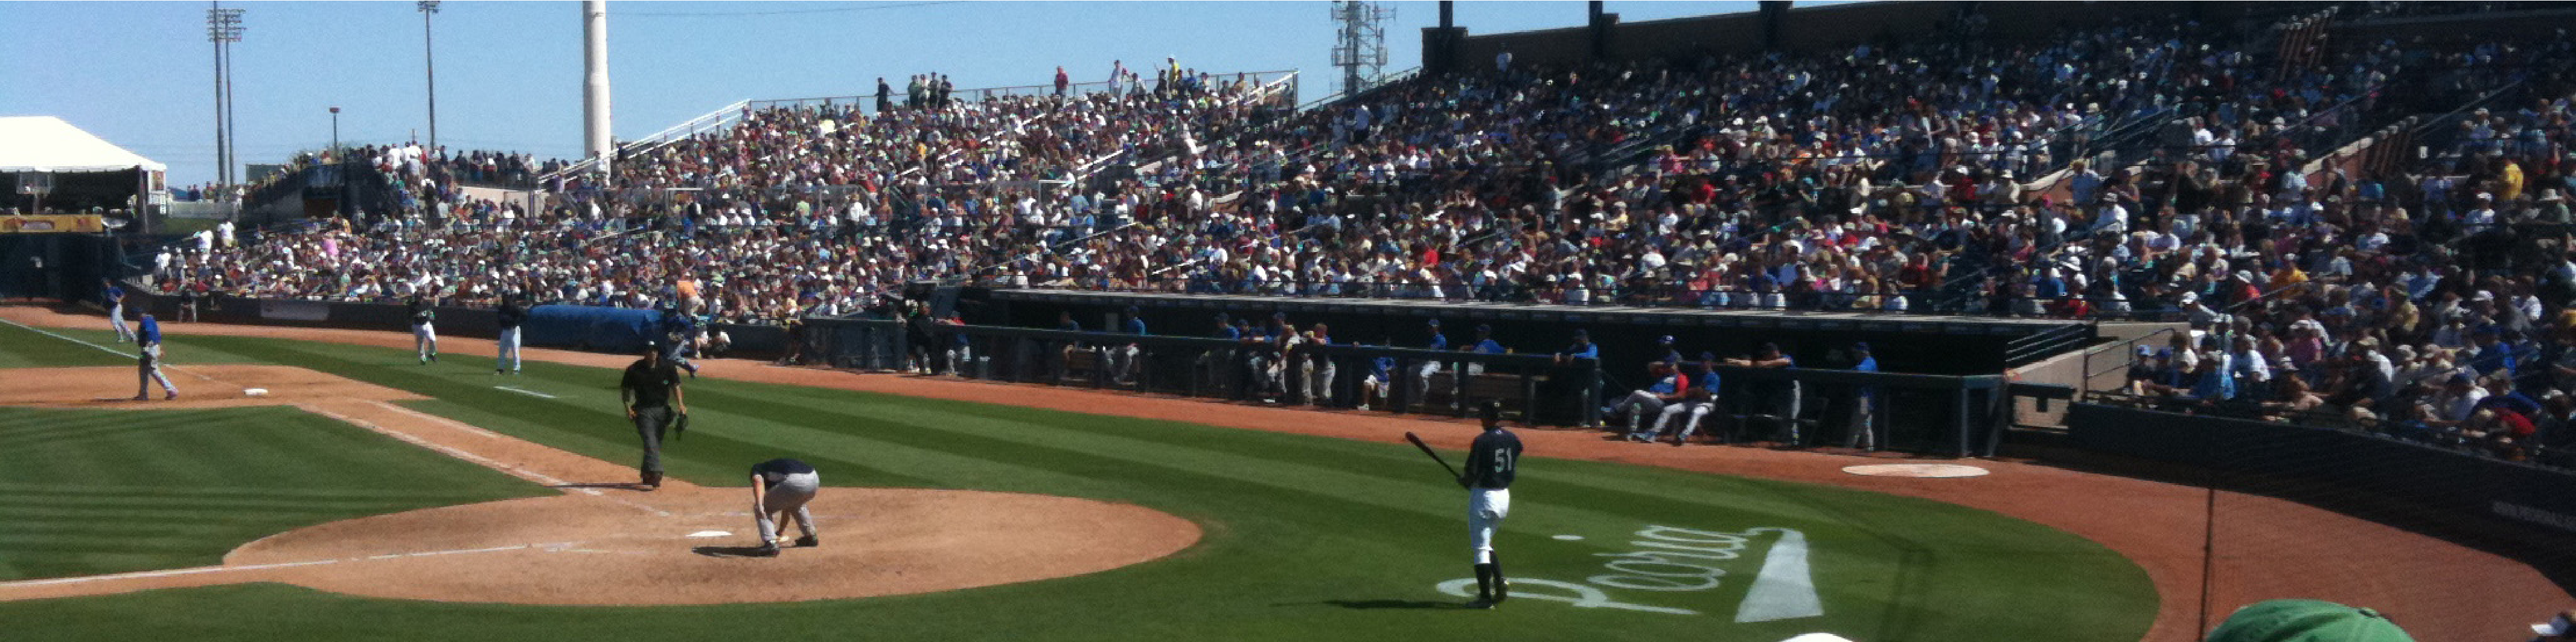
\includegraphics[width=\textwidth]{sampleteaser}
%  \caption{Seattle Mariners at Spring Training, 2010.}
%  \Description{Enjoying the baseball game from the third-base
%  seats. Ichiro Suzuki preparing to bat.}
%  \label{fig:teaser}
%\end{teaserfigure}

%% 盲审：接收/修订/录用日期仅用于正式出版稿，审稿提交时请保持注释。
%\received{20 February 2007}
%\received[revised]{12 March 2009}
%\received[accepted]{5 June 2009}

%%
%% This command processes the author and affiliation and title
%% information and builds the first part of the formatted document.
\maketitle

\section{Introduction}

Large Language Models (LLMs) have rapidly evolved from standalone research artifacts 
into the computational backbone of diverse intelligent applications. Modern 
LLM-based Agent systems (e.g., multi-turn chatbots, autonomous code generation 
pipelines, and large-scale document processing workflows) inherently orchestrate 
multiple inference calls into structured, multi-step execution graphs. As these 
deployments scale from research prototypes to production services handling 
thousands of concurrent workflows, the efficiency of the underlying inference 
infrastructure has emerged as a critical bottleneck. In this context, the 
global scheduler within a multi-tenant LLM serving cluster assumes 
a critical role: it must simultaneously dictate the execution priority 
of pending requests and route them to optimal backend instances, 
with the primary objective of minimizing end-to-end workflow latency 
under highly dynamic and heterogeneous workloads.

Classical scheduling strategies designed for stateless, single-turn inference 
fall short in these dynamic scenarios, as they rely on assumptions that Agent 
workloads inherently contradict. First, Agent workflows feature dynamic, nonlinear 
topologies, such as conditional branches and iterative repair loops. Because 
actual execution paths and depths are resolved only at runtime, static graph-based 
priority estimation becomes ineffective. Second, requests generated across different 
stages of a single workflow are heterogeneous in input/output lengths and GPU 
memory footprints. Consequently, uniform scheduling treatment typically induces 
head-of-line blocking and resource imbalance. Third, adjacent calls within a workflow 
contain overlapping context prefixes. This presents KV cache reuse opportunities, 
forcing a strict trade-off between cache locality and cluster-wide load balancing.

Existing approaches only partially address these scheduling challenges. On the queuing 
side, FCFS remains unaware of workflow progress, propagating queuing delays along dataflow 
edges. Topology-aware strategies like Ayo~\cite{tan2025towards} prioritize requests 
based on static residual stage counts. However, they become ineffective when dynamic 
branches and loops cause the estimated stage depth to deviate from the actual execution 
trajectory. On the routing front, Round-Robin policies achieve load balance at the expense 
of prefix-cache locality. Conversely, Session Affinity, as adopted by end-to-end systems 
such as Parrot~\cite{lin2024parrot}, maximizes cache reuse via static session binding. 
Yet, this approach induces hardware hotspots when parallel fan-out stages concentrate requests 
on a single instance, and it lacks the adaptability to handle dynamic load shifts, frequently 
resulting in cluster-wide load imbalances. Taken together, these limitations indicate that 
effective global scheduling for LLM Agent serving necessitates the co-design of queuing and routing 
algorithms, as neither tier can achieve robust performance in isolation.

In response to these challenges, we present \textbf{RAGS} (\underline{R}L-based \underline{A}gent 
\underline{G}lobal \underline{S}cheduler), a co-designed global scheduling framework that 
addresses both queuing and routing dimensions in a coordinated manner. The queuing layer, \textbf{DynA}, 
determines request priorities using exclusively runtime-observable signals (specifically, online-estimated completion-round distributions, 
accumulated workflow latencies, and per-request queue ages), operating independently of any 
predefined workflow topology. Concurrently, the routing layer employs a Reinforcement Learning 
(RL) policy that models request-to-instance assignment as a Markov Decision Process. By training 
a Transformer-based network via Double-DQN, it jointly optimizes KV cache reuse, cluster load balance, 
and queue congestion, ensuring continuous adaptability through offline pretraining coupled with online 
fine-tuning.

The main contributions of this paper are as follows.
\begin{itemize}
  \item We propose an adaptive queuing algorithm that estimates the overall completion 
        probability of active workflows using statistics gathered at runtime. 
        By prioritizing individual requests based on the execution progress of their 
        parent workflows, this approach effectively mitigates head-of-line blocking among 
        concurrent tasks.

  \item To the best of our knowledge, RAGS is the first to apply reinforcement learning 
        to global routing in LLM Agent serving. By jointly encoding heterogeneous cluster features, 
        including KV cache states, load distributions, and GPU hardware configurations, 
        the RL policy realizes an adaptive, multi-objective routing strategy that strictly 
        outperforms traditional static heuristics.

  \item Evaluations on a simulated LLM serving cluster demonstrate that RAGS reduces mean 
        end-to-end workflow latency by up to \textbf{5.2$\times$} compared to a normal  
        Round-Robin baseline, and by \textbf{3--4$\times$} against Parrot and Ayo. Furthermore, 
        ablation studies and experiments on heterogeneous GPU clusters validate the individual 
        effectiveness and hardware adaptability of the co-designed queuing and routing modules.
\end{itemize}

\section{Background and Problem Analysis}
\label{sec:background-and-problem-analysis}

Conventionally, LLM serving systems employ a layered scheduling architecture in which 
the global scheduler manages two interconnected operations: (1) determining 
the execution priority of pending requests, and (2) routing each request to an 
appropriate backend instance. This section characterizes the distinctive structural 
properties of LLM Agent workloads to demonstrate why conventional request-level 
heuristics prove inadequate for these tasks. By exposing these systemic limitations, 
we motivate the necessity of the comprehensive global scheduling framework detailed 
in Section~\ref{sec:system-design}, which systematically addresses both the queuing 
and routing dimensions.

\subsection{Characteristics of LLM Agent Workflows}
\label{subsec:agent-workflow}

To systematically characterize LLM Agent workloads, we surveyed mainstream open-source projects 
on GitHub~\cite{aws2026genaichatbot,cognitivetech2026ollama,opencode2026terminal} and 
analyzed representative paradigms, including chatbots, code generation, and document 
summarization. As illustrated in Figure~\ref{fig:agent-dag}, a typical Agent workflow 
can be abstracted as a directed graph. In this structural model, each node represents 
an individual LLM inference call or tool invocation, while each edge encodes a specific 
dataflow or control dependency. Based on this analysis, we identify three distinctive 
system-level traits inherent to Agent workloads.

\begin{figure}[t]
  \centering
  % 倒三角形：上排 (a)(b)，下排 (c) 居中
  \begin{subfigure}[c]{0.48\linewidth}
    \centering
    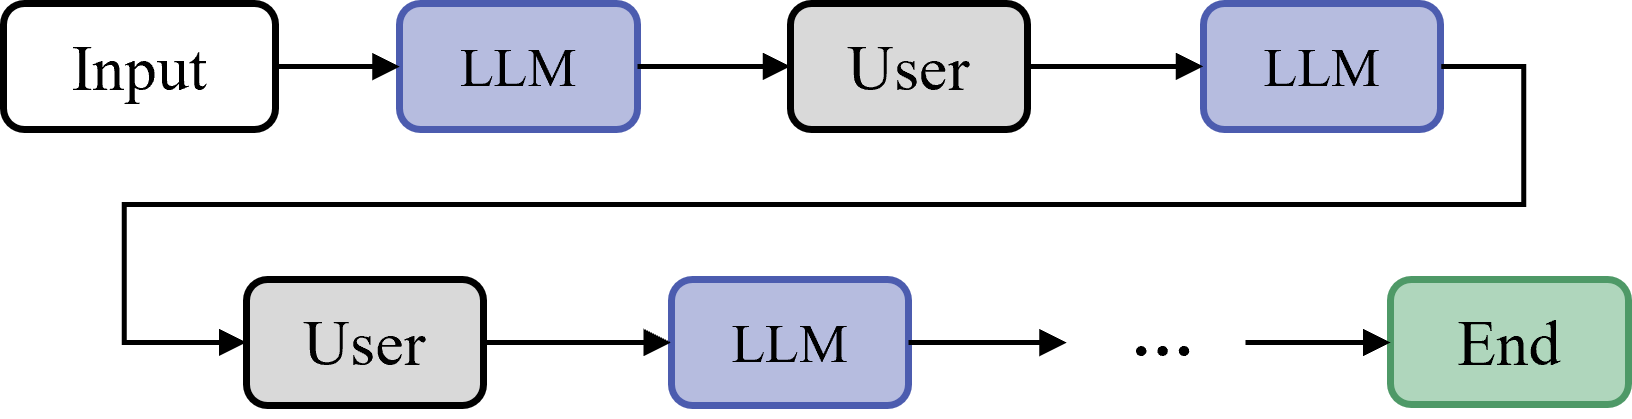
\includegraphics[width=\textwidth]{../figures/2.1.a.png}
    \caption{Chatbot.}
    \label{fig:agent-dag-a}
  \end{subfigure}
  \hfill
  \begin{subfigure}[c]{0.48\linewidth}
    \centering
    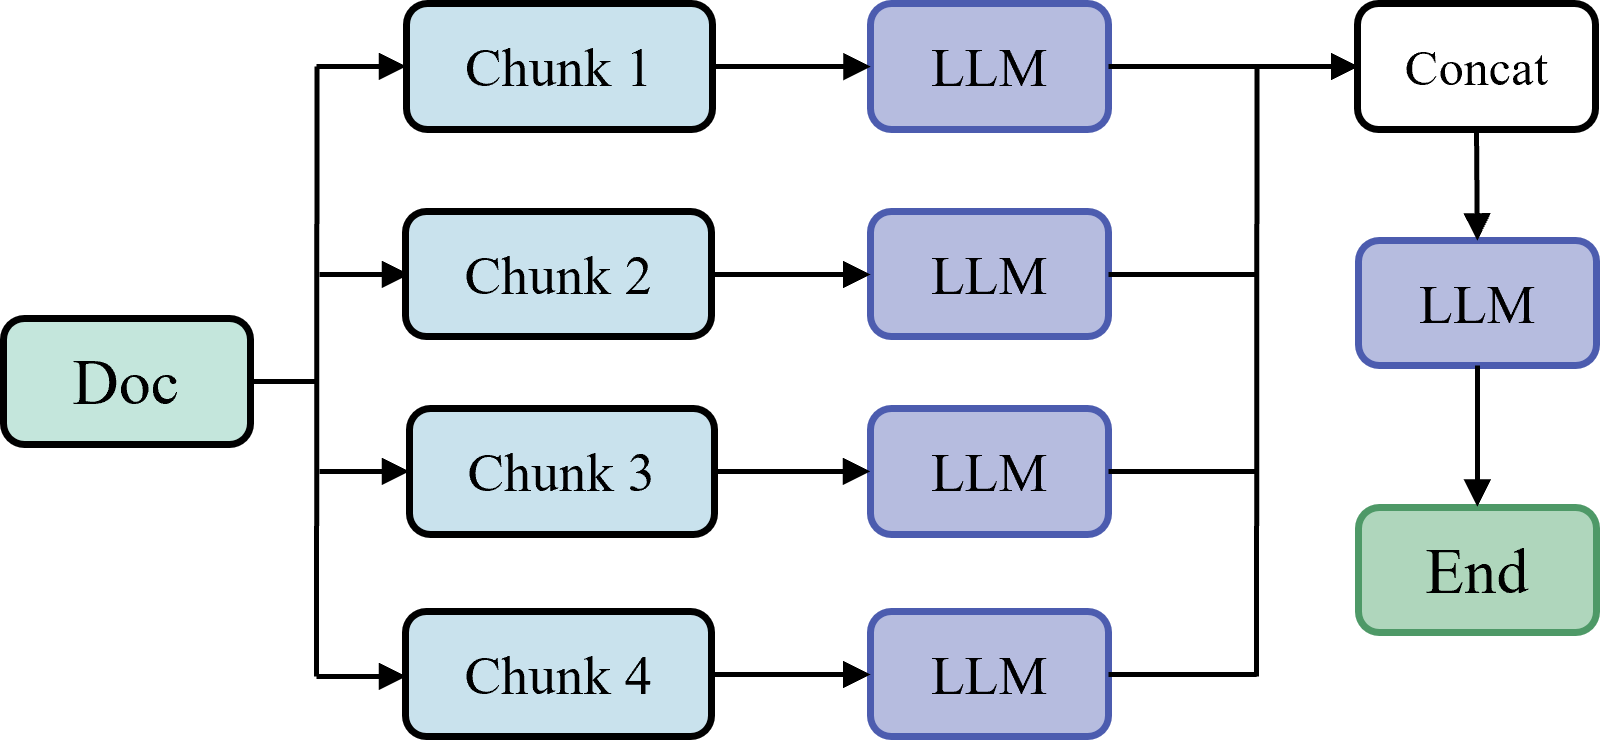
\includegraphics[width=\textwidth]{../figures/2.1.b.png}
    \caption{Map-Reduce document summarization.}
    \label{fig:agent-dag-b}
  \end{subfigure}

  \vspace{0.5cm}

  \null\hfill
  \begin{subfigure}[b]{0.48\linewidth}
    \centering
    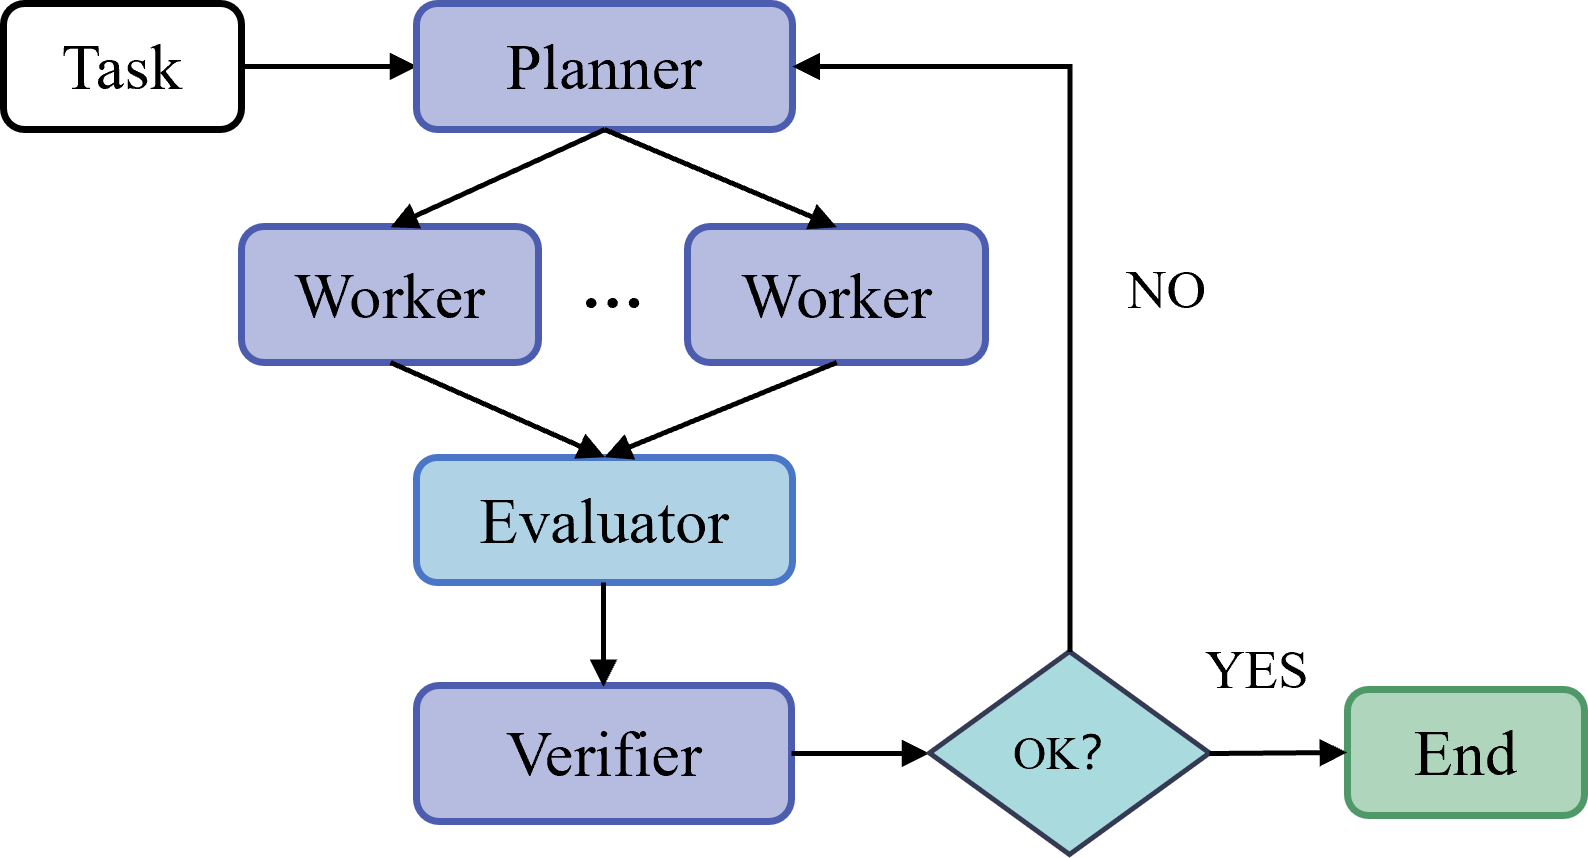
\includegraphics[width=\textwidth]{../figures/2.1.c.png}
    \caption{Code generation.}
    \label{fig:agent-dag-c}
  \end{subfigure}
  \hfill\null
  \caption{Representative LLM Agent workflow structures.}
  \label{fig:agent-dag}
\end{figure}

\textbf{Dynamic, nonlinear topologies with mixed concurrency.}
Agent workflows incorporate conditional branches, feedback loops, and interleaved
sequential and parallel stages (e.g., iterative repair cycles and Map-phase fan-outs).
Consequently, these features result in dynamically changing execution paths, rendering 
static graph-based scheduling approaches ineffective.

\textbf{Heterogeneous inference costs across workflow nodes.}
Nodes serving different roles (such as routing, generation, and quality review) emit 
requests with varying prompt lengths, output lengths, and execution latencies. 
Because these resource requirements can differ by over $25\times$ within a single 
application~\cite{chen2025kairos}, scheduling decisions must be strictly cost-aware.

\textbf{Deep context sharing and KV cache affinity.}
Adjacent calls within the same workflow contain overlapping context prefixes, 
presenting KV cache reuse opportunities. However, affinity-driven routing inherently 
concentrates requests and induces node-level hotspots, forcing a strict trade-off 
between cache locality and cluster-wide load balancing.

Taken together, these architectural traits inherently contradict the classical assumption 
of independent, homogeneous requests. The following two subsections examine the concrete 
limitations that arise when standard queuing and routing policies are applied to Agent 
workloads.

\subsection{Limitations of Existing Queuing Algorithms}
\label{subsec:queue-challenges}

Conventional LLM serving paradigms model requests as independent, single-turn calls, 
where FCFS queuing is sufficient for fairness. Agent workloads, 
however, comprise interdependent requests that introduce three fundamental scheduling 
challenges.

\noindent\textbf{(1) Head-of-line blocking from workflow progress heterogeneity.}
Concurrent Agent requests exhibit varying execution progress, meaning the system 
simultaneously processes initial LLM calls and near-terminal tasks. Because FCFS 
is progress-agnostic, it frequently stalls near-completion requests behind newly 
admitted early-stage tasks, directly inflating end-to-end workflow latencies.

\noindent\textbf{(2) Cascading amplification and accumulation of queuing delays.}
Queuing delays experienced at any individual node propagate along dataflow dependencies. 
Furthermore, because FCFS ranks requests solely by arrival time, it ignores accumulated 
workflow-level latencies. Consequently, tail performance degrades as delays compound 
across successive stages.

\noindent\textbf{(3) Inability to handle dynamic workflow topologies.}
Topology-aware strategies like Ayo~\cite{tan2025towards} prioritize tasks with fewer 
remaining stages based on a static workflow graph. However, when dynamic branches or 
loops execute at runtime, the statically estimated residual stage counts deviate from 
actual execution paths, causing tasks within active loops to be improperly 
under-prioritized.

Collectively, these limitations necessitate an adaptive queuing policy that tracks 
actual workflow progress and accumulated latencies independent of static topologies.

\subsection{Limitations of Existing Routing Strategies}
\label{subsec:routing-challenges}
\begin{figure}[h]
  \centering
  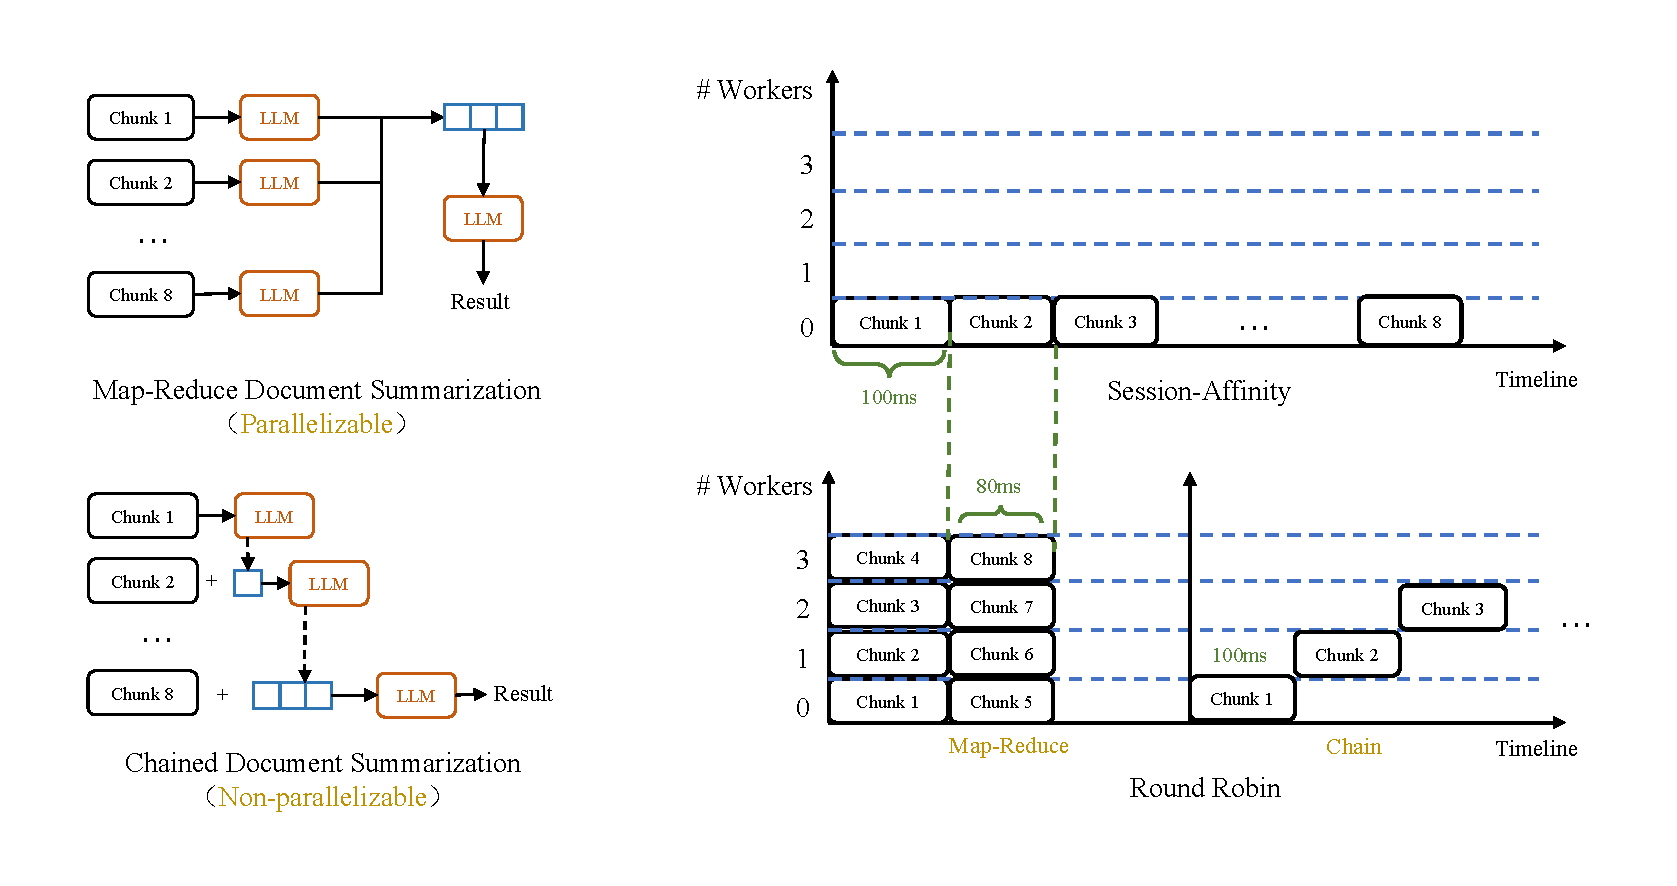
\includegraphics[width=\linewidth]{../figures/2.3.pdf}
  \caption{RR versus Session Affinity under parallel and sequential
    document-summarization Agent workflows.}
  \Description{Placeholder for the figure comparing Round-Robin and Session
    Affinity across parallel and sequential workflow shapes.}
  \label{fig:routing-motivation}
\end{figure}

Conventional global routing mechanisms for LLM serving typically utilize 
Round-Robin (RR) to distribute requests sequentially for load balancing, 
or Session Affinity (SA) to bind session requests to a fixed instance for 
maximizing KV cache reuse. However, both strategies exhibit structural 
limitations when processing Agent workloads.

\textbf{RR ignores request heterogeneity.} 
Because requests from distinct functional nodes exhibit diverse context 
lengths and GPU memory footprints, RR's uniform routing often concentrates 
memory-intensive tasks on a single instance. This concentration saturates 
GPU memory and triggers request preemptions. Consequently, preempted tasks 
incur re-queuing and recomputation overheads, directly degrading overall 
system throughput.

\textbf{SA mishandles intra-workflow concurrency.} 
During parallel execution stages (e.g., the Map phase in document 
summarization), workflows emit numerous concurrent subtask requests. 
By binding all these requests to a single instance, SA creates local 
hardware hotspots while leaving other instances underutilized, thereby 
compromising cluster-wide load balancing.

As illustrated in Figure~\ref{fig:routing-motivation}, RR achieves 
lower latency on parallel workflows by exploiting 
cluster-wide concurrency, whereas SA outperforms RR on sequential 
workflows by preserving KV cache locality across stages. 
Because neither policy dominates universally, the optimal routing choice 
depends jointly on execution topologies, temporal dependencies, and 
real-time cache states.

To address these limitations, recent systems incorporate richer heuristics, 
such as multi-objective linear weighting~\cite{srivatsa2024preble}. 
However, LLM cluster states evolve continuously: request arrival patterns, 
instance queue lengths, and memory utilization fluctuate rapidly. Furthermore, 
each routing decision reshapes the environment encountered by subsequent 
requests. Static, fixed-weight heuristics lack the agility to capture these 
complex state transitions or to optimize the trade-off between immediate 
scheduling gains and long-horizon throughput.

Collectively, the isolated failures of existing queuing and routing algorithms 
necessitate the holistic global scheduling framework detailed in 
Section~\ref{sec:system-design}.

\section{Algorithm Design}\label{sec:system-design}

\subsection{System Architecture}
\label{subsec:rags-arch}

Figure~\ref{fig:rags-arch} illustrates the overall system architecture 
and request processing pipeline of RAGS. The system frontend accepts 
heterogeneous Agent workflows and forwards all LLM inference requests 
to the global scheduler for centralized management. Within the scheduler, 
requests first enter the global queue, where the adaptive queuing module, 
\textbf{DynA}, calculates priorities and reorders pending tasks. 
Subsequently, the RL-driven routing policy asynchronously assigns these 
requests to target instances by evaluating queue characteristics alongside 
cluster states. Following inference completion, the system triggers 
subsequent workflow stages. Concurrently, backend instances continuously 
report load metrics back to the scheduler to maintain an 
accurate environmental state. Once the workflow concludes, the system returns 
the final result to the user.
\begin{figure}[h]
  \centering
  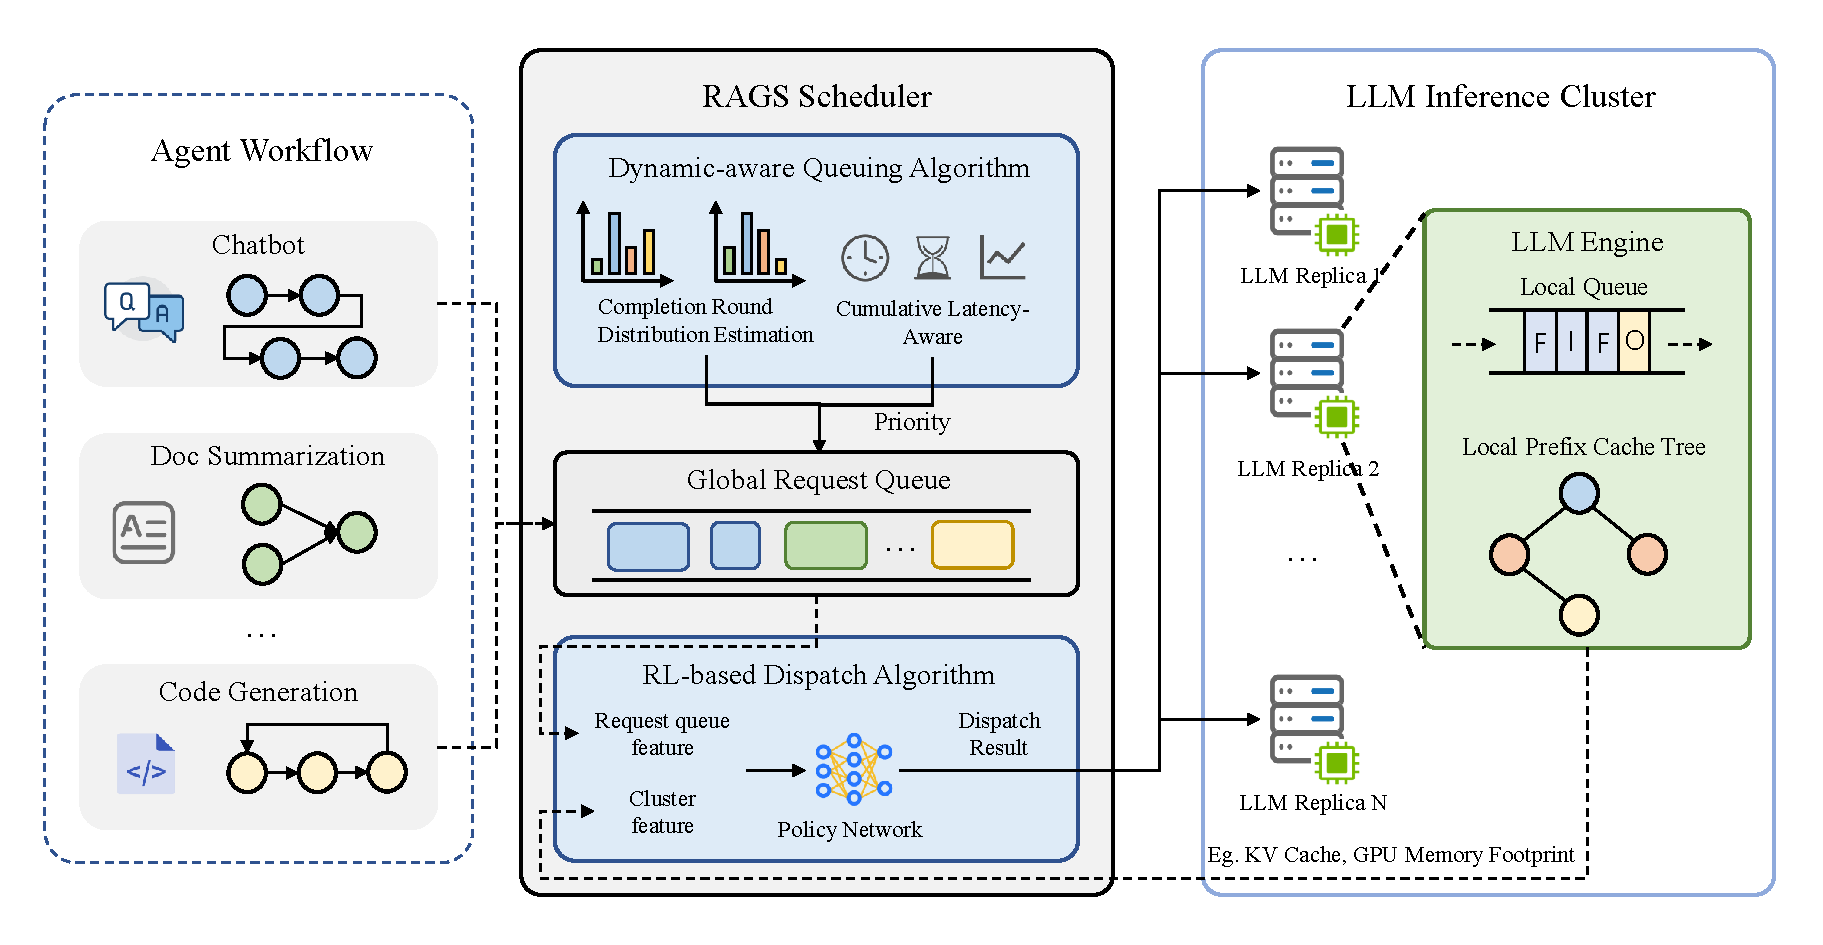
\includegraphics[width=\linewidth]{../figures/3.1.pdf}
  \caption{RAGS system architecture.}
  \label{fig:rags-arch}
\end{figure}

%Based on this architecture, we elaborate on the two core
%components, namely the queuing algorithm and the dispatch algorithm,
%in the following subsections.
Building upon this architectural overview, the following subsections detail 
the two core scheduling components: the queuing algorithm and the routing policy.

\subsection{DynA: Dynamic-Aware Queuing Algorithm}\label{sec:queue-algorithm}
Due to the dynamic branching and autoregressive uncertainty inherent in Agent 
workflows, traditional queuing policies that rely on static topologies 
prove inadequate. These methods assume a priori knowledge of the workflow structure, 
a condition rarely satisfied in actual deployments.

To overcome this reliance, we introduce \textbf{DynA} 
(\underline{Dyn}amic-\underline{A}ware Queuing). The core principle 
of DynA is to derive all priority decisions exclusively from runtime-observable 
signals, including online-estimated completion-round distributions, accumulated 
workflow latencies, and per-request queue ages. By doing so, it operates entirely 
independently of predefined workflow topologies. Specifically, the algorithm 
functions across two dimensions: inter-Agent priority ordering governed 
by actual workflow progress, and intra-Agent request ordering driven by 
accumulated latencies.

\subsubsection{Workflow-Progress-Aware Inter-Agent Priority}
\label{subsec:inter-agent}

To differentiate the execution progress of requests from different
Agent types (and thus prioritize requests in the later stages of
their workflows) without knowing the workflow topology, DynA
introduces an \emph{online completion round distribution} mechanism.

Let $F_a(n)$ denote the empirical CDF of completion rounds for Agent
type $a$, i.e., the probability that the total number of LLM calls in
any completed workflow instance of this type does not exceed $n$. This
distribution is maintained at runtime by continuously collecting
statistics from completed workflows, without any prior assumption
about static workflow topology.

Specifically, each time an Agent workflow of type $a$ completes, the
system records the completion round count $n_j$ and updates $F_a(n)$
via Exponential Moving Average (EMA):
\begin{equation}
  \label{eq:ema-update}
  F_a^{(t+1)}(n) = (1-\lambda)\cdot F_a^{(t)}(n) + \lambda\cdot\mathbb{1}[n_j \le n],
\end{equation}
where $\lambda \in (0,1)$ is the smoothing coefficient and
$\mathbb{1}[\cdot]$ is the indicator function. By assigning higher
weight to recent observations, EMA enables $F_a(n)$ to adapt to
dynamic workload changes while filtering out stale historical data.

For Agent types with no historical records, the system initializes
$F_a$ with a uniform prior on $[1, N_{\max}]$:
\[
  F_a(n) = \begin{cases}
    0,            & n < 1 \\
    n/N_{\max},   & 1 \le n \le N_{\max} \\
    1,            & n > N_{\max}
  \end{cases}.
\]
During online operation, EMA drives this prior toward the true
empirical distribution.

Based on this real-time empirical distribution, when the scheduler
receives a request from Agent type $a$ that has already completed $k$
LLM calls, it computes the \emph{conditional near-completion
probability} $\hat{P}_{a,k}$, defined as the probability of reaching the
terminal state within the next $\Delta$ calls given that $k$ calls
have already been made:
\begin{equation}
  \label{eq:conditional-prob}
  \hat{P}_{a,k} = P(k \le N_a \le k{+}\Delta \mid N_a \ge k)
                = \frac{F_a(k{+}\Delta) - F_a(k{-}1)}{1 - F_a(k{-}1)},
\end{equation}
where $N_a$ is the random variable representing total LLM calls for
Agent type $a$, and $\Delta$ is a look-ahead window size (default
$\Delta{=}1$). A larger $\hat{P}_{a,k}$ indicates a higher probability
of near-term completion, so DynA assigns higher scheduling priority to
requests with larger $\hat{P}_{a,k}$. This design borrows from the
Shortest Job First (SJF) principle while avoiding any dependence on a
priori topology.

\subsubsection{Cumulative-Latency-Aware Intra-Agent Ordering}
\label{subsec:intra-agent}

For concurrent requests of the same type and same round, DynA applies
an intra-Agent ordering strategy based on workflow start time. Let
$t_r^{\text{start}}$ be the initial trigger time of the workflow
containing request $r$; the system prioritizes requests with earlier
$t_r^{\text{start}}$, compensating requests that have already
accumulated longer delays.

To prevent starvation of long-horizon Agent types under this
priority ordering, DynA introduces a queue-age-aware anti-starvation
mechanism. Define the current queuing wait time of request $r$ as
$\tau_r = t_{\text{current}} - t_r^{\text{arrive}}$. When $\tau_r$
reaches a system-defined maximum tolerance threshold $\tau_{\max}$,
the following priority boost is triggered:
\begin{equation}
  \label{eq:age-boost}
  \text{Boost}(r) = \max\!\left(0,\;\frac{\tau_r - \tau_{\max}}{\tau_{\max}}\right).
\end{equation}

Combining the conditional near-completion probability with the
anti-starvation mechanism, DynA computes a comprehensive priority
score for each queued request $r$:
\begin{equation}
  \label{eq:priority-score}
  \text{Score}(r) = \hat{P}_{a_r, k_r} + \eta \cdot \text{Boost}(r),
\end{equation}
where $a_r$ is the Agent type of $r$, $k_r$ is the total LLM call
count so far for the workflow instance, and $\eta$ is the
anti-starvation weight hyperparameter. Requests with higher scores are
scheduled first; ties are broken by Agent start time. The complete
DynA policy is given in Algorithm~\ref{alg:dyna}.

\begin{algorithm}
  \caption{Dynamic-Aware Queuing Algorithm (DynA)}
  \label{alg:dyna}
  \begin{algorithmic}[1]
    \REQUIRE Request queue $Q$; online completion-round distributions
             $\{F_a\}$; anti-starvation threshold $\tau_{\max}$;
             weight $\eta$
    \ENSURE  Next request to dispatch $r^*$
    \FOR{each request $r \in Q$}
      \STATE Retrieve Agent type $a_r$ and completed call count $k_r$
      \IF{$F_{a_r}$ is not yet initialized}
        \STATE $F_{a_r}(n)\leftarrow \min(n,N_{\max})/N_{\max}$
               \quad\textit{// uniform prior}
      \ENDIF
      \STATE $\hat{P}_{a_r,k_r}\leftarrow
             \dfrac{F_{a_r}(k_r{+}\Delta)-F_{a_r}(k_r{-}1)}
                   {1-F_{a_r}(k_r{-}1)}$
      \STATE $\tau_r \leftarrow t_{\text{current}} - t_r^{\text{arrive}}$
      \STATE $\text{Boost}(r)\leftarrow
             \max\!\left(0,\;\dfrac{\tau_r-\tau_{\max}}{\tau_{\max}}\right)$
      \STATE $\text{Score}(r)\leftarrow
             \hat{P}_{a_r,k_r} + \eta\cdot\text{Boost}(r)$
    \ENDFOR
    \STATE Sort all requests in $Q$ by
           $\bigl(\text{Score}(r)\;\text{desc},\;
                  t_r^{\text{start}}\;\text{asc}\bigr)$
    \STATE $r^*\leftarrow$ first request in $Q$
    \RETURN $r^*$
  \end{algorithmic}
\end{algorithm}

\subsection{RL-based Dispatch Algorithm}
\label{sec:rl-dispatch}

\subsubsection{Problem Formulation and MDP Definition}
\label{subsec:mdp}

We formalize the global scheduler's dispatch process as a Markov
Decision Process (MDP) and solve for the optimal dispatch policy using
reinforcement learning. 
%Key symbols are summarized in
%Table~\ref{tab:chapter4-symbols}.

% \begin{table}
%   \caption{Notation for the global dispatch problem.}
%   \label{tab:chapter4-symbols}
%   \begin{tabular}{ll}
%     \toprule
%     Symbol      & Definition \\
%     \midrule
%     $K$         & Number of LLM instances \\
%     $M$         & LLM model type \\
%     $G$         & GPU type \\
%     $N$         & Total number of Agent workflows \\
%     $Q_t$       & Set of pending requests at time $t$ \\
%     $r_j$       & The $j$-th request in the global queue \\
%     $w_i$       & The $i$-th Agent workflow \\
%     $q_{i:k}$   & The $k$-th request of workflow $w_i$ \\
%     $l_i$       & End-to-end completion time of $w_i$ \\
%     $s_{t:i}$   & The $i$-th sub-state of the cluster at time $t$ \\
%     $a_t^i$     & The $i$-th dispatch action at time $t$ \\
%     \bottomrule
%   \end{tabular}
% \end{table}

Consider a service system with $K$ homogeneous LLM instances, each
equipped with GPU $G$ and deploying model $M$. During system
operation, $N$ Agent workflows arrive online over time. At any
decision step $t$, let $Q_t$ denote the set of pending requests in
the global scheduler. The scheduler assigns a target LLM instance
$a_t$ to each request $q_{i:k}$ (the $k$-th call of workflow $w_i$).
The optimization objective is to minimize the average end-to-end
latency across all $N$ workflows:
\begin{equation}
  \min_{a_t}\;\frac{1}{N}\sum_{i=1}^{N} l_i,
\end{equation}
where $l_i$ is the actual end-to-end completion time of $w_i$.

Since $Q_t$ may contain multiple concurrent requests, a centralized
joint assignment would require an action space of $O(|Q_t|\!\times\!K)$.
To avoid the curse of dimensionality, we adopt a progressive decision
paradigm: the agent assigns one request at a time to a target
instance.

The MDP is defined as follows. Every $\Delta t$, the global scheduler
determines target LLM instances for all requests in the waiting queue.
At step $t$, the agent observes state $s_{t:j}$ and outputs a
discrete action $a_t^j \in \{1,\ldots,K\}$, routing the $j$-th
queued request $r_j$ to the $a_t^j$-th LLM instance.

\begin{figure}[h]
  \centering
  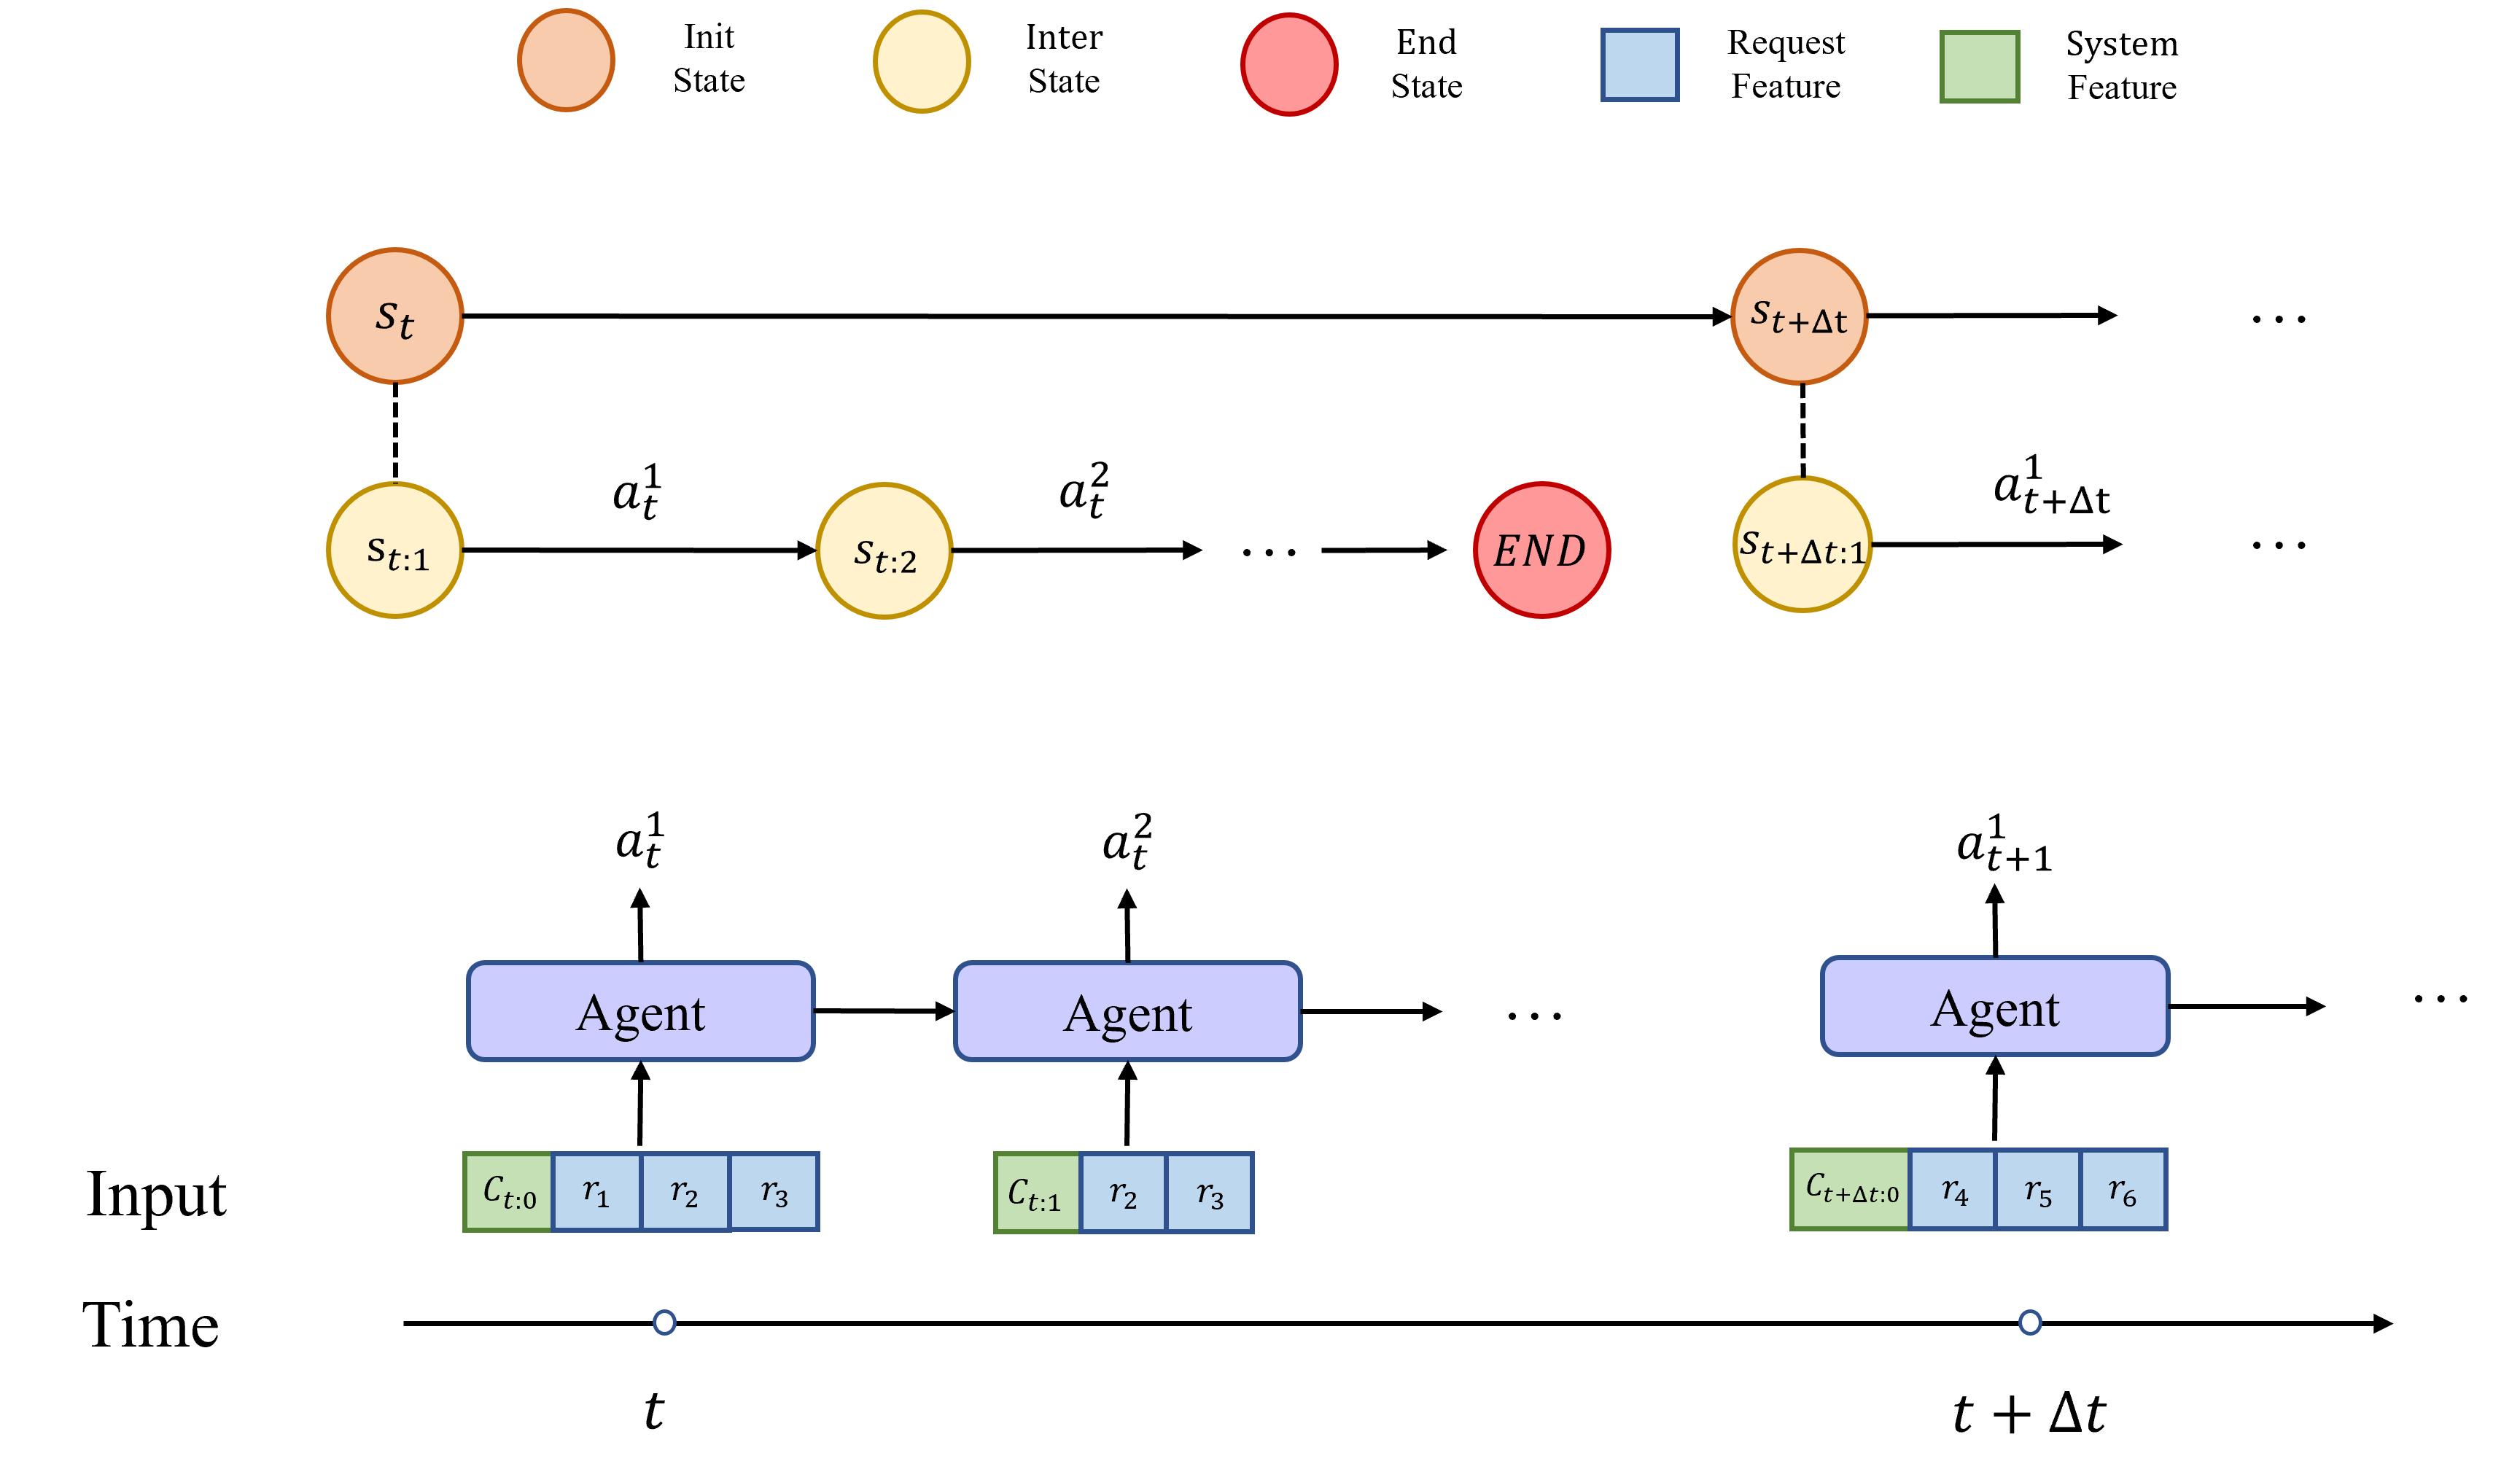
\includegraphics[width=\linewidth]{../figures/3.2.png}
  \caption{Markov Decision Process for global dispatch.}
  \Description{Placeholder for the MDP diagram.}
  \label{fig:chap4-mdp}
\end{figure}

\subsubsection{State Space}

The state $s_t$ encodes the current global system state, comprising
features of the pending request set and the load status of each LLM
instance.

\textbf{Request state.} The matrix $\mathbf{X}_t^{req}$ comprises four distinct feature vectors:
\begin{itemize}
\item $\vec{p}$ is the input length vector, where $p_i$ denotes the number of input tokens for the $i$-th queued request.
\item $\vec{d}$ is the estimated output length vector, where $d_i$ represents the predicted output length of the $i$-th request.
\item $\vec{u}$ is the parallel-stage indicator vector, where $u_i \in \{0, 1\}$ flags whether the $i$-th request resides in a parallelizable workflow stage.
\item $\vec{\kappa}$ is the workflow type vector, where $\kappa_i$ uniquely identifies the Agent application class of the $i$-th request.
\end{itemize}

Regarding the estimated output length $d_i$, we follow the methodology in~\cite{jin2023s} 
by predicting discrete length intervals rather than exact token counts. 
This coarse-grained approximation proves sufficient, as our designed MDP relies solely 
on relative interval magnitudes. Empirical evaluations demonstrate an 
interval prediction accuracy of approximately 70\%.

\textbf{Cluster state.} The matrix $\mathbf{X}_t^{inst}$ is constructed by 
concatenating individual per-instance feature vectors. Specifically, 
the runtime profile of each LLM instance is characterized by:
\begin{itemize}
  \item $\vec{m}$ and $\vec{g}$: One-hot encoded vectors specifying the instance's deployed 
  model architecture and underlying GPU hardware, respectively.
  \item $\vec{wq}$: A load histogram of the waiting queue, derived by binning input lengths 
  with a configurable step size $\mathit{bin\_width}$.
  \item $\vec{rq}$: A load histogram of active execution queues. Prefill-stage requests 
  are binned by input token length, whereas Decode-stage requests are binned by estimated 
  output length.
  \item $c$: GPU memory utilization, computed as the proportion of allocated KV-cache blocks 
  to the total block capacity.
  \item $s$: The expected prefix-cache reuse rate for the pending request, 
  quantified as the fraction of reusable tokens.
  \item $b$: The estimated batch execution latency, maintained via a sliding-window 
  average of recent iteration times.
\end{itemize}

To ensure training stability, all features are strictly normalized. 
The comprehensive MDP state representation is thus formulated as 
$s_t = [\mathbf{X}_t^{req} \,\|\, \mathbf{X}_t^{inst}]$, where $\,\|\,$ 
denotes the concatenation operator.

\subsubsection{Reward Function}

Using the end-to-end workflow latency directly as a reward signal
would cause severe reward sparsity and credit-assignment problems due
to the asynchronous execution model of LLM inference systems. Instead,
we design a \emph{composite immediate reward} that provides feedback
after every dispatch decision:
\begin{equation}
  \label{eq:dispatch-reward}
  r_t = \lambda_k\cdot r_k + \lambda_{imb}\cdot r_{imb}
       + \lambda_p\cdot r_p + \lambda_T\cdot T(x_{t,i}^{inst}),
\end{equation}
where the terms are:
\begin{itemize}
  \item $r_k$: \emph{Prefix cache reuse reward}, representing the expected
        KV-cache reuse rate on the target instance, encouraging lower
        time-to-first-token.
  \item $r_{imb}$: \emph{Load-imbalance penalty}, measuring the
        impact of the current dispatch on global load uniformity.
  \item $r_p$: \emph{Queue penalty}, equal to the current waiting-queue
        length of the target instance, discouraging dispatch to overloaded
        nodes.
  \item $T(x_{t,i}^{inst})$: \emph{Throughput estimate}, denoting the
        expected token throughput of the target instance in its current state.
\end{itemize}

To quantify load imbalance $r_{imb}$, the total load of instance $i$
is estimated from its active request distribution ($\vec{rq}$) and
waiting queue distribution ($\vec{wq}$):
\begin{equation}
  L_i = \sum_{j=1}^{N_{bin}}\bigl(C_j\cdot N_{run,j}\bigr)
       + \sum_{j=1}^{N_{bin}}\bigl(C_j\cdot N_{pend,j}\bigr),
\end{equation}
where $C_j$ is the center length of bin $j$ and $N_{\cdot,j}$ is the
count of requests in that bin. The normalized imbalance score is:
\begin{equation}
  S_{imb} = \frac{\sum_{i=1}^{K}|L_i - \bar{L}|}
                 {\sum_{i=1}^{K} L_i + \epsilon},
\end{equation}
with $\bar{L} = \frac{1}{K}\sum_i L_i$ and $\epsilon$ a small
constant for numerical stability. We set $r_{imb} = -S_{imb}$.

For the throughput estimate $T(x_{t,i}^{inst})$, we train a
lightweight neural network surrogate offline on tens of thousands of
real scheduling trajectories using MSE loss, achieving approximately
10\% prediction error.

\subsubsection{Policy Network Architecture}
\label{subsec:policy-net}

To capture complex temporal dependencies and heterogeneous instance
features, we design a \emph{Transformer-based scheduling network} that
jointly encodes the current target request, the waiting-queue context,
and the real-time state of each instance.
Figure~\ref{fig:dispatch-policy-net} shows the network topology.

\begin{figure}[h]
  \centering
  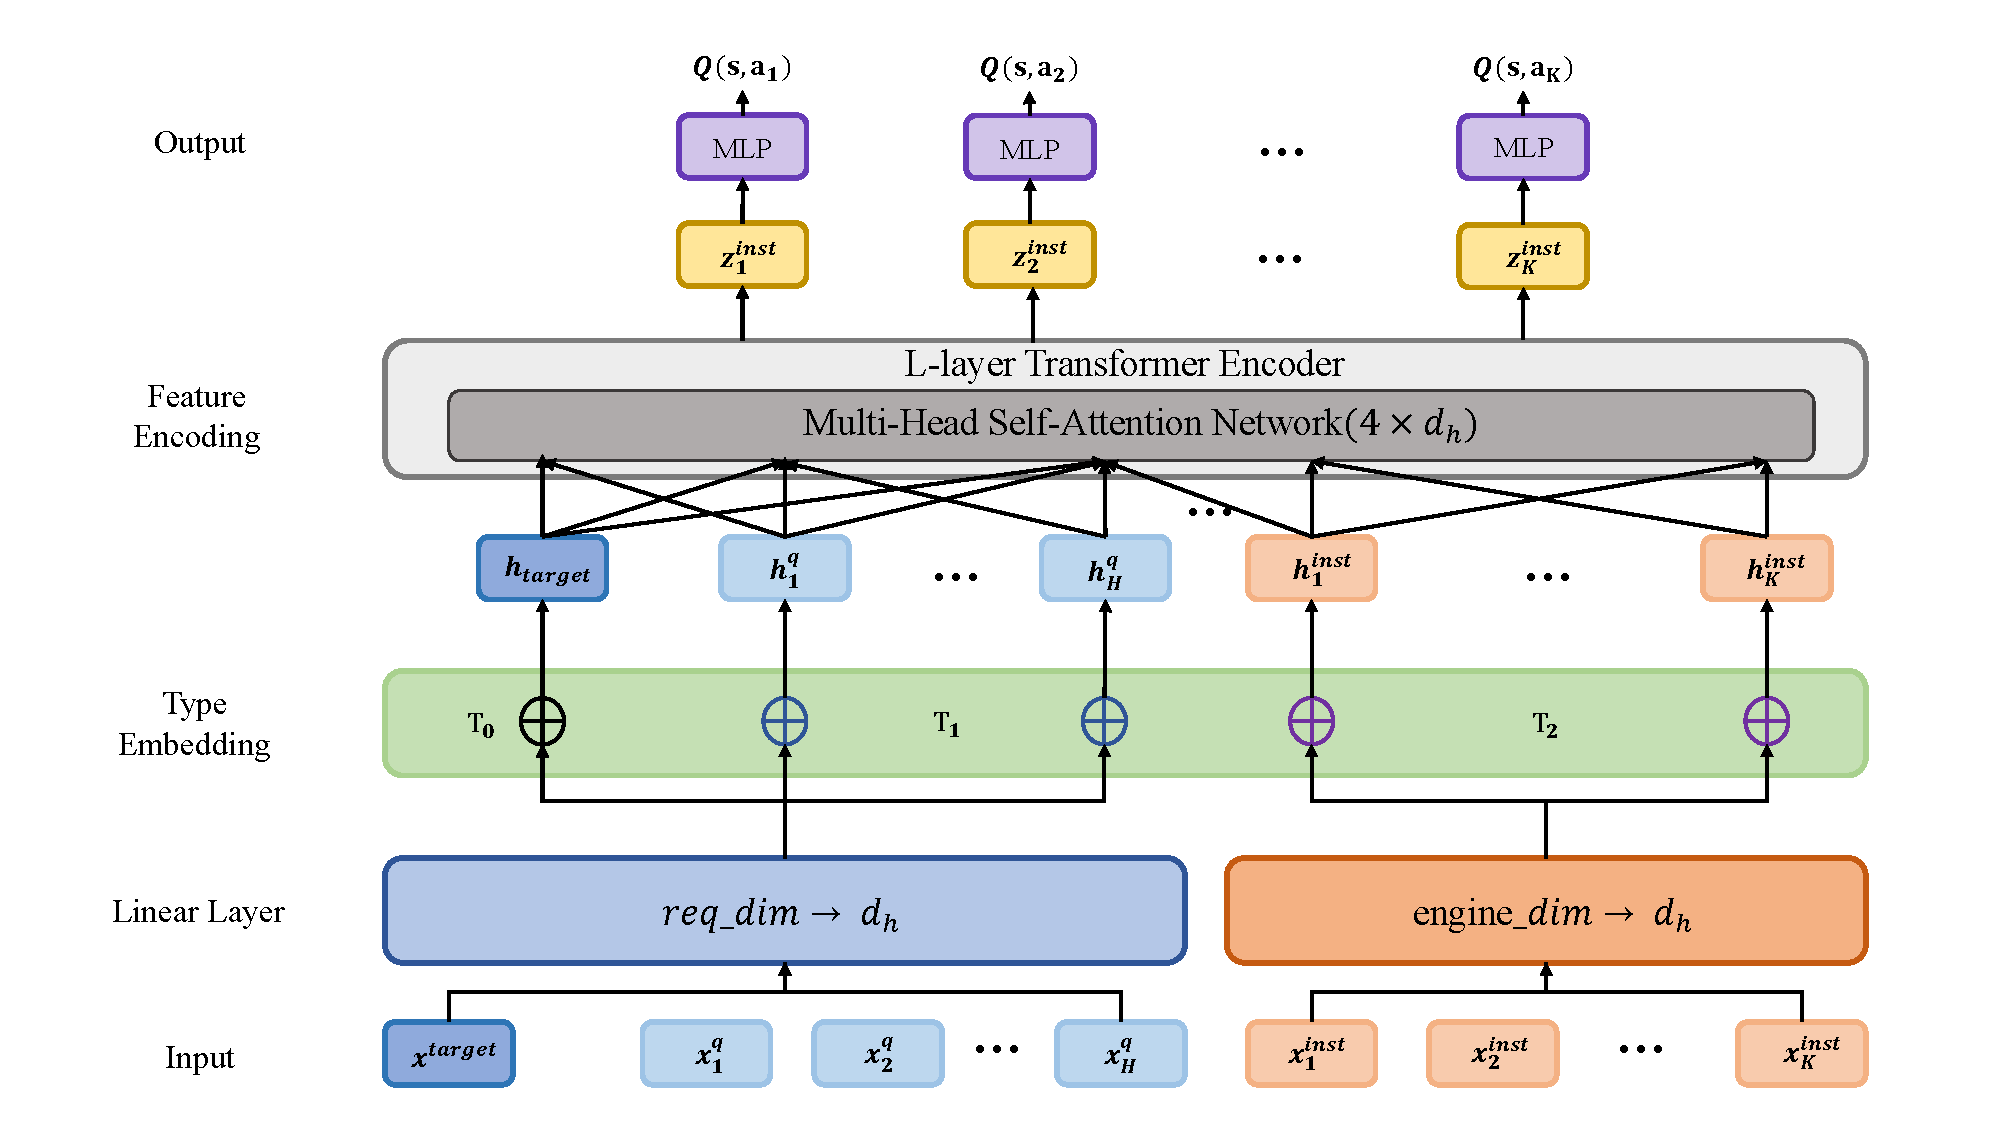
\includegraphics[width=\linewidth]{../figures/3.3.pdf}
  \caption{Dispatch policy network architecture.}
  %\Description{Placeholder for the policy network architecture diagram.}
  \label{fig:dispatch-policy-net}
\end{figure}

The input layer is divided into three feature subspaces: the current
target request $\mathbf{x}^{target}$, a look-ahead waiting queue
$\{\mathbf{x}^q_i\}_{i=1}^H$ of length $H$, and the real-time states
of $K$ LLM instances $\{\mathbf{x}^{inst}_j\}_{j=1}^K$.
Each feature vector is first projected to a unified hidden dimension
$d_h$ via a linear layer, then augmented with learned type embeddings
to distinguish target, queue, and instance tokens
($\text{type}\in\{0,1,2\}$).
The resulting sequence is processed by $L$ Transformer encoder layers
to capture cross-token dependencies.
At the output layer, we extract the $K$ instance-token
representations $\{\mathbf{z}_{inst,j}\}_{j=1}^K$ and map each to an
action-value score via a shared-parameter $Q$-value head:
\begin{equation}
  Q(s,a_j) = \mathbf{W}_Q\cdot\text{ReLU}
             \!\left(\mathbf{W}_H\mathbf{z}_{inst,j}+\mathbf{b}_H\right)+b_Q.
\end{equation}
The final output $\mathbf{Q}\in\mathbb{R}^K$ gives the expected
cumulative return for dispatching the current request to each
instance.

\subsubsection{Reinforcement Learning Training}
\label{sec:training}

We adopt a two-phase scheme combining offline pretraining and online
fine-tuning.

\textbf{Offline Pretraining.}
We construct a data-driven offline simulation environment by replaying
real production workload traces covering diverse Agent workflows (e.g.,
multi-turn dialogue, code generation, document summarization) at
various load intensities, improving generalization.

For the high-dimensional discrete action space, we adopt the
\emph{Double-DQN} algorithm~\cite{van2016deep}, which decouples
target action selection from value estimation to suppress Q-value
overestimation. 
%Its target is:
%\begin{equation}
%  \label{eq:ddqn-target}
%  Y_t^{DDQN} = r_t + \gamma\,Q\!\left(s_{t+1},
%               \arg\max_{a'}Q(s_{t+1},a';\theta_t);\,\theta_t^-\right),
%\end{equation}
%where $\theta_t$ is the online network (action selection) and
%$\theta_t^-$ is the target network (value evaluation). 
We replace the original MSE loss with Huber Loss~\cite{huber1992robust}, which
applies linear penalty for large TD errors, significantly improving
training stability under heterogeneous request sequences.

\textbf{Online Fine-tuning.}
Although offline training establishes baseline scheduling capabilities, 
static policies often suffer performance degradation in highly dynamic production clusters. 
Consequently, we introduce an online fine-tuning mechanism. The agent continuously records 
interaction transitions into an experience replay buffer, triggering periodic parameter 
updates at a low learning rate once a predefined sample threshold is reached. 
To maintain Quality of Service stability, we bound the $\epsilon$-greedy exploration rate 
and employ momentum-based soft updates for the target network, effectively mitigating 
Q-value oscillations under distribution shifts.

\section{Implementation}\label{sec:implementation}

To support RL agent training and system evaluation, we build our testbed upon 
Vidur~\cite{agrawal2024vidur}, an open-source LLM inference simulator. 
Vidur natively supports heterogeneous GPUs (e.g., A100, H100) and provides 
built-in benchmarks for mainstream models like Llama and Qwen, enabling rapid 
validation of scheduling algorithms across diverse configurations.

However, native Vidur primarily targets single-turn LLM requests. 
It lacks the capability to simulate the multi-step interaction dependencies 
inherent in Agent workflows, nor does it support prefix-cache reuse. 
To address these limitations, we augment Vidur's core engine along two dimensions:

\subsection{KV Cache Reuse}

To enable KV cache reuse within the LLM engine (i.e., the local scheduler), 
we implement a \texttt{tree\_cache} module atop Vidur's native \texttt{memory\_pool}. 
This module comprises two core components: a \emph{Block Manager} responsible for 
the allocation and reclamation of memory blocks, and a \emph{Local Prefix Cache Tree} 
that maintains the prefix-mapping relationships of KV caches within each LLM instance.

Unlike sglang's single-level prefix tree, our design maintains both a
per-instance local tree and a cluster-wide global tree augmented with
replica mappings to enable cross-instance KV cache reuse.
As shown in Figure~\ref{fig:tree-cache-total}, different request
prefixes branch from the root node. Each node stores the token
sequence, a reference count (\texttt{ref}) for memory reclamation, and
a block index (\texttt{block}) mapping to the KV store.

To integrate with PagedAttention, only block-aligned prefixes are
treated as valid cache entries, ensuring consistency with the
underlying paged memory manager.

\begin{figure}[t]
  \centering
  \begin{subfigure}[t]{0.49\linewidth}
    \centering
    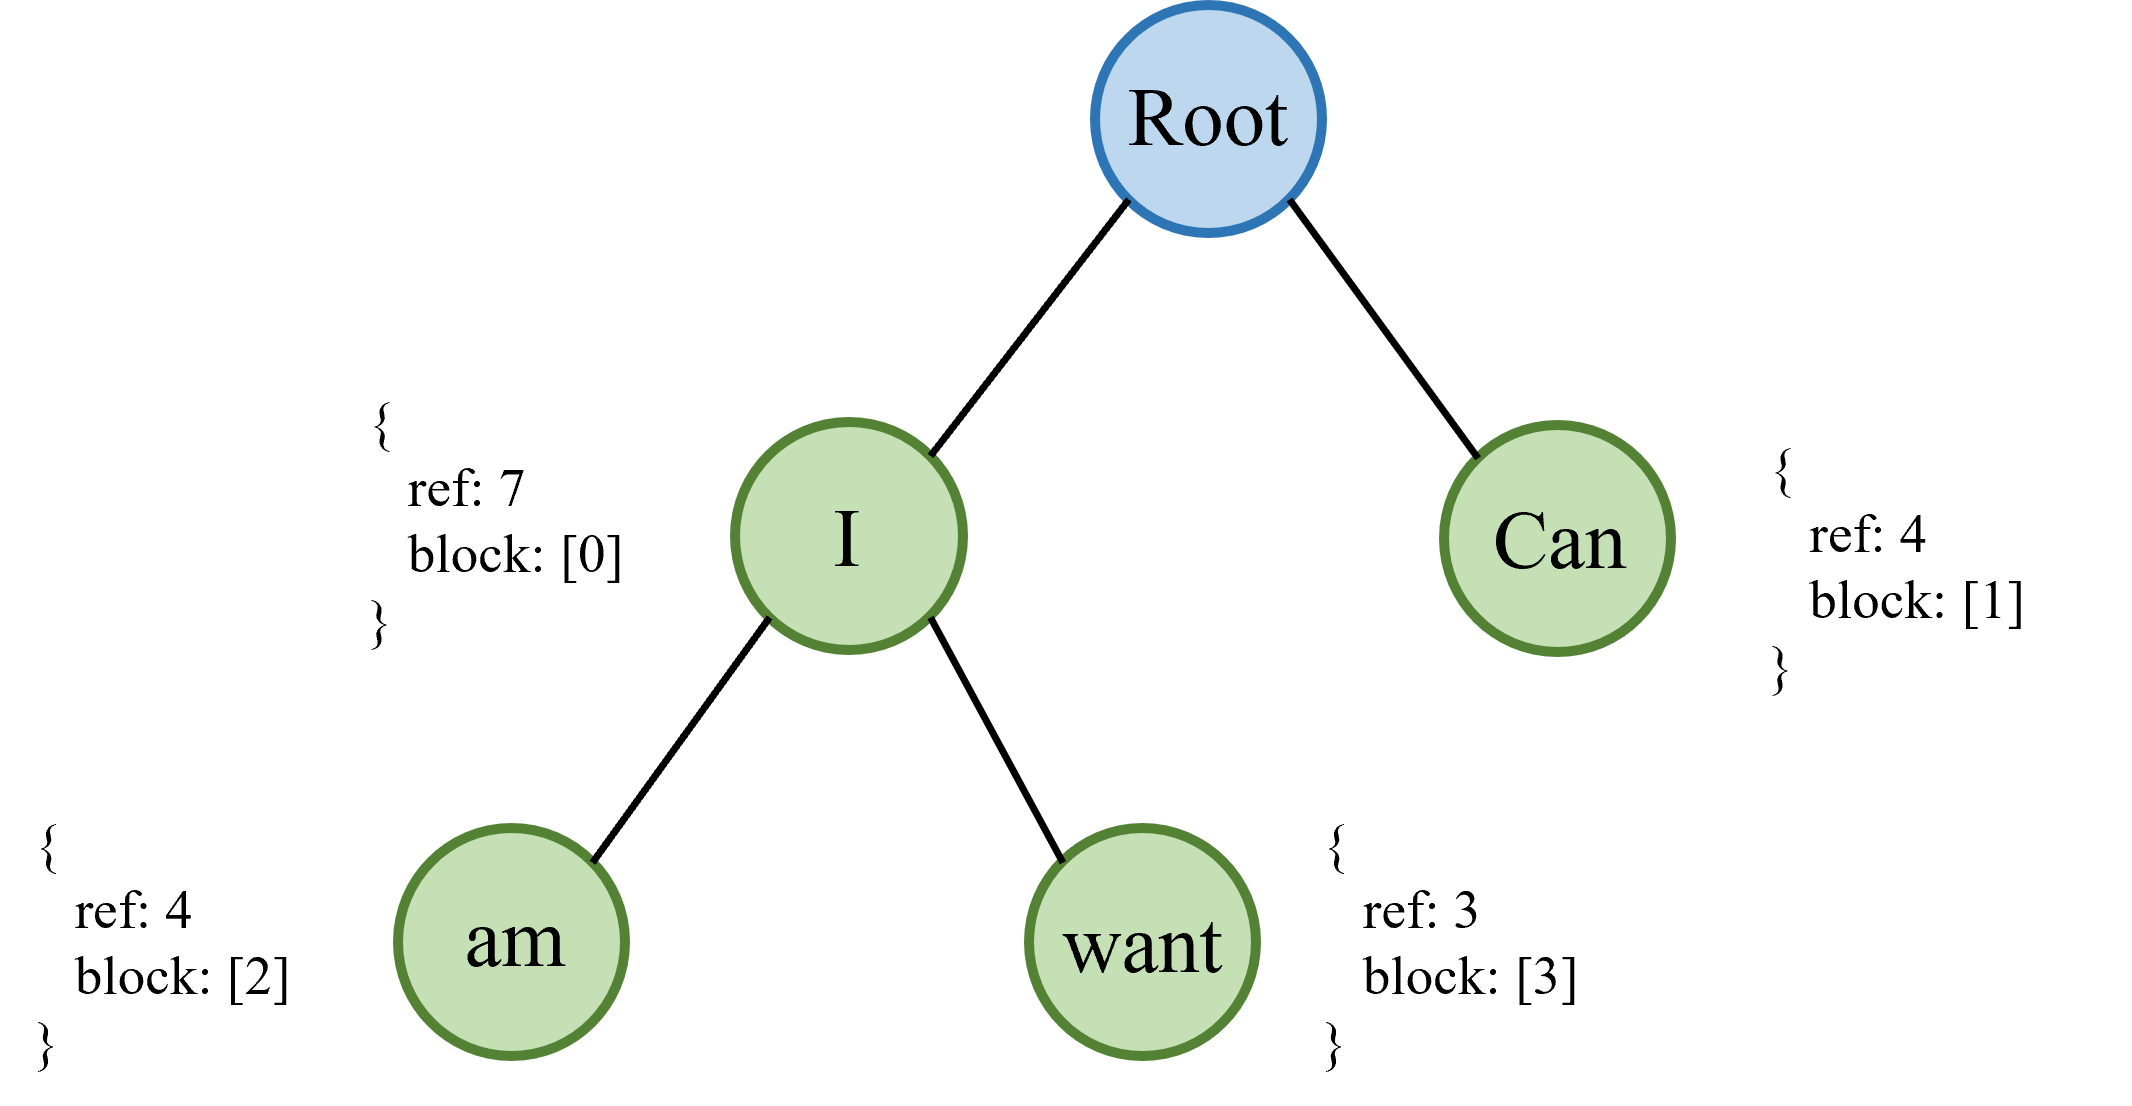
\includegraphics[width=\linewidth,height=0.22\textheight,keepaspectratio]{../figures/4.1.a.png}
  \end{subfigure}\hfill
  \begin{subfigure}[t]{0.49\linewidth}
    \centering
    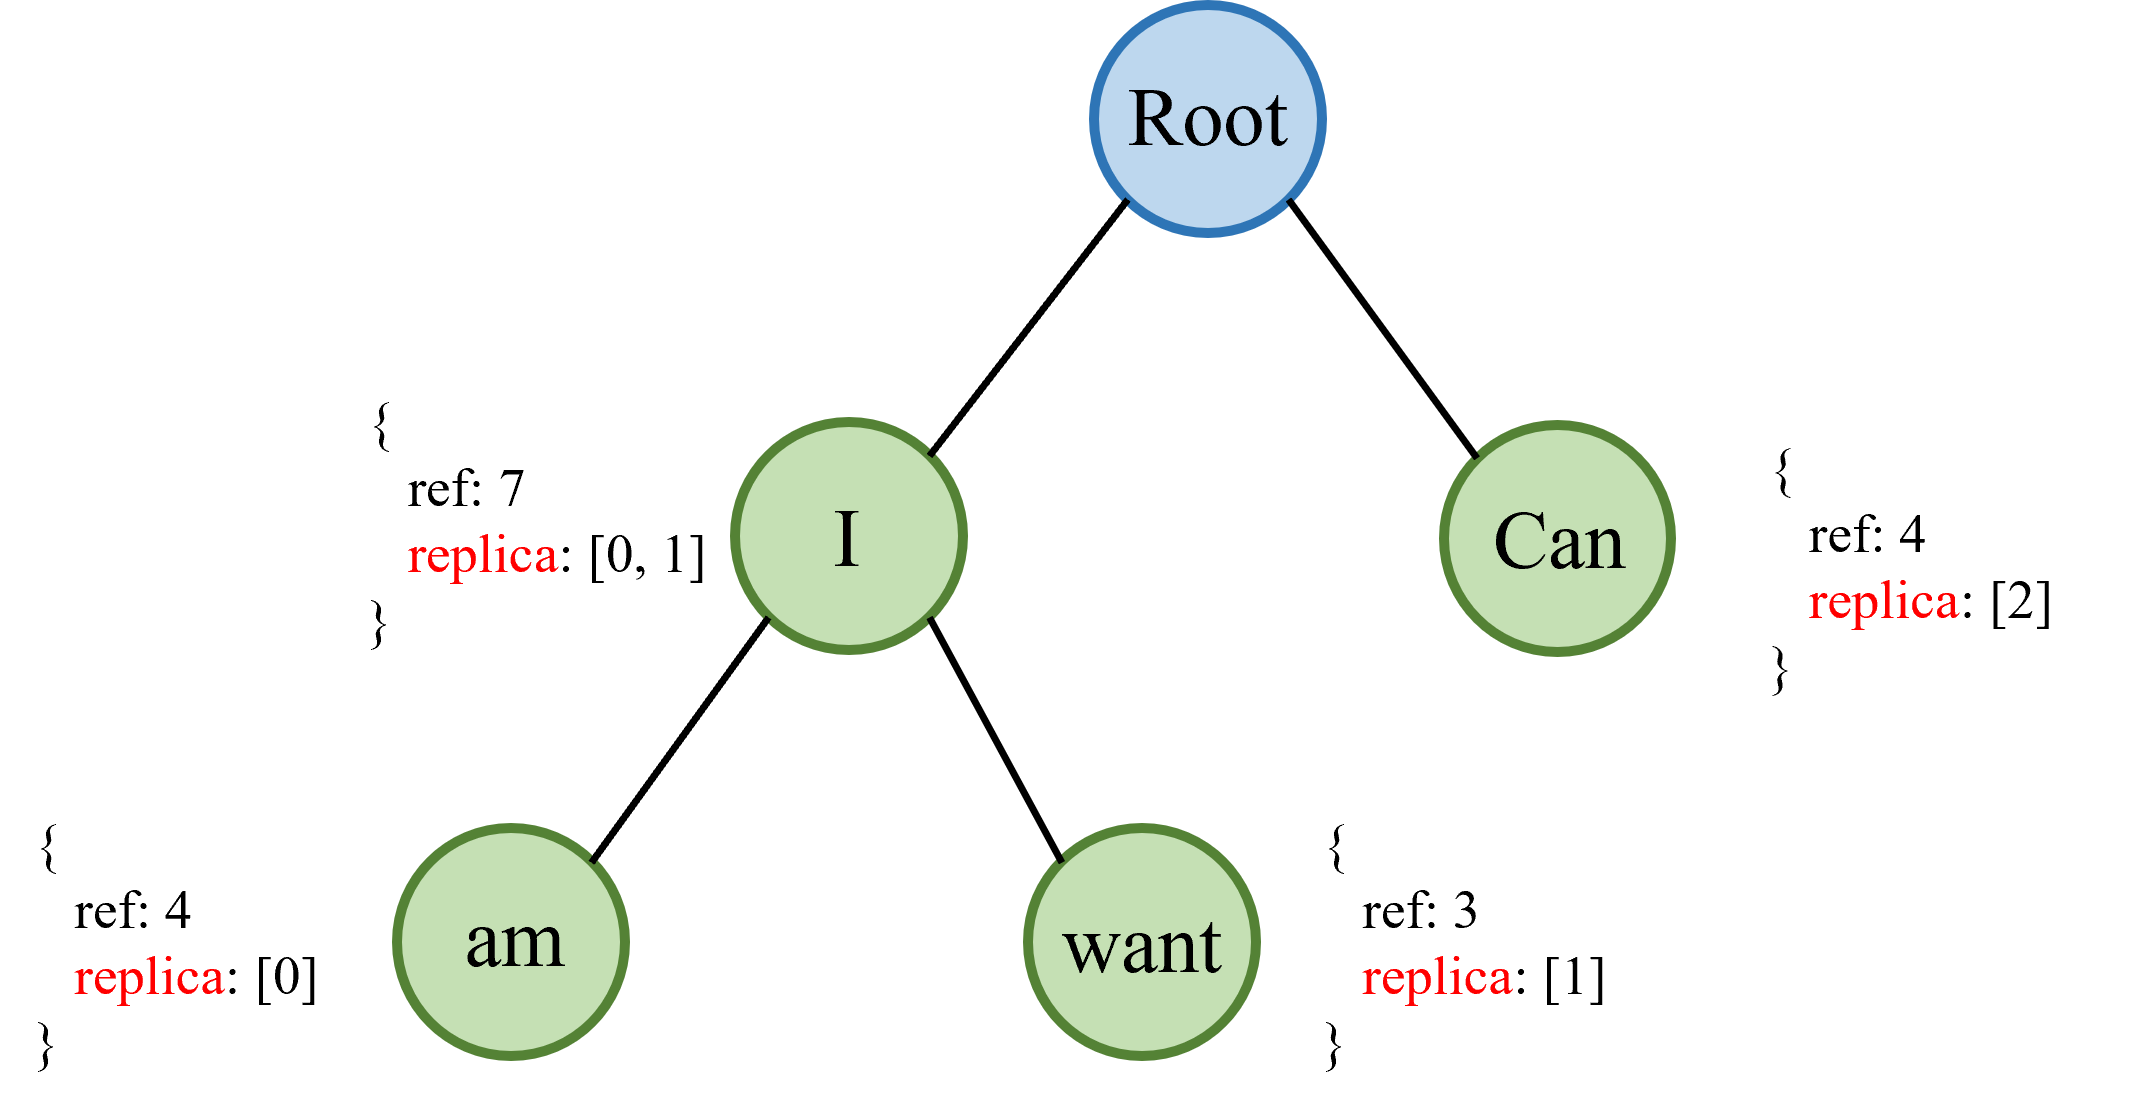
\includegraphics[width=\linewidth,height=0.22\textheight,keepaspectratio]{../figures/4.1.b.png}
  \end{subfigure}
  \caption{KV cache prefix trees: local (left) and global (right).}
  \Description{KV cache prefix trees: local tree (left) and global tree
    (right).}
  \label{fig:tree-cache-total}
\end{figure}

The \emph{global KV cache prefix tree}, maintained by the global
scheduler, records cache states across all LLM instances. Its structure
mirrors the local tree, with the sole difference that each node stores
a mapping from tree nodes to LLM instances (\texttt{replica}). When a
user request arrives, the global scheduler can quickly locate matching
instances through this tree, enabling cross-instance KV cache reuse.

\subsection{Agent Workflow Support}

Since Vidur cannot directly simulate complex Agent workflow logic, we
extend it with a \texttt{UnifiedRequest} class that inherits from
\texttt{Request} and adds \texttt{agent\_type} and \texttt{agent\_id}
metadata for workflow identification.

\texttt{UnifiedRequest} further encodes a \emph{workflow graph} of
call-chain dependencies: subsequent stage requests are activated only
after all predecessor requests in the graph have completed, faithfully
simulating serial and parallel multi-step Agent interactions.


\section{Evaluation}\label{sec:evaluation}

\subsection{Experimental Setup}

\subsubsection{Hardware and Software Environment}
All model training and experimental evaluation are conducted on a
physical server running Ubuntu 18.04.6 LTS, equipped with dual Intel
Xeon E5-2680 v3 processors (2.50\,GHz) and two NVIDIA GeForce RTX
3090 GPUs.

For inference simulation we use the Vidur simulator. We emulate a
four-node LLM inference cluster in which each node is equipped with a
40\,GB NVIDIA A100 GPU and independently deploys one
Meta-Llama-3-8B instance. The prefill chunk size (\texttt{chunk\_size})
is set to 4096 and the maximum batch capacity (\texttt{batch\_size})
to 512.

Agent workflows are implemented with the LangChain
framework~\cite{langchain} to generate realistic request sequences and
workflow topologies for the experiments.

\subsubsection{RL Training Configuration}
We set the learning rates for offline pretraining and online fine-tuning to $5\times10^{-5}$ 
and $1\times10^{-5}$, respectively, with a discount factor $\gamma = 0.995$. 
The experience replay buffer is configured with a maximum capacity of 50,000 samples 
and a warm-up period of 500 samples. During training, the policy network, 
which features a hidden dimension of 512, is optimized using mini-batches of 256 samples. 
To ensure stability, the target network is updated every 100 steps, while the 
$\varepsilon$-greedy exploration rate is linearly decayed from 0.5 to 0.01.

For DynA, we set the look-ahead window $\Delta=1$, the anti-starvation
threshold $\tau_{\max}=10.0$\,s, and $\eta=0.1$.

\subsubsection{Agent Workloads}
To comprehensively evaluate the proposed method across different Agent
workflow types, we select three representative LLM Agent workloads
covering serial, parallel, and hybrid topologies.
Figure~\ref{fig:four-images-total} shows the token-length and
request-count distributions of each workload.

\textbf{ChatBot (serial).}
We build approximately 8\,000 multi-turn dialogue workflows from the
ShareGPT dataset~\cite{chiang2023vicuna}, each containing 2--20
dialogue rounds. The input length follows a right-skewed distribution
(mean $\approx$837.54 tokens, concentrated in 0--2000 tokens), while
output lengths are more concentrated (mean $\approx$191.78 tokens),
reflecting the long-input/short-output pattern of conversation tasks.

\textbf{Map-Reduce Summarization (parallel).}
We construct a Map-Reduce document summarization Agent: the Map phase
splits long documents into chunks and issues concurrent LLM requests
for sub-summaries; the Reduce phase aggregates them into a final
output. Using the Wikidata dataset~\cite{vrandevcic2014wikidata}, we
build approximately 1\,000 workflows with 2--50 LLM requests each. The
mean input length is $\approx$833.51 tokens with higher variance than
ChatBot, and the mean output length is $\approx$186.51 tokens.

\textbf{Code Generation Agent (hybrid).}
We design a multi-stage Agent following the pipeline
User $\to$ Planner $\to$ Workers $\to$ Evaluators $\to$ Verifier $\to$
Final Output. If the code fails evaluation, a feedback loop triggers
the Planner to re-schedule Workers for iterative repair. Using
HumanEval~\cite{chen2021evaluating} and
MBPP~\cite{austin2021program}, we build $\approx$1\,000 workflows with
2--50 LLM requests each. The mean input length is $\approx$3541.76
tokens (significantly higher than the other two workloads, due to the
feedback repair context), and the mean output length is
$\approx$800.87 tokens.

\begin{figure*}[t]
  \centering
  \begin{subfigure}[t]{0.23\textwidth}
    \centering
    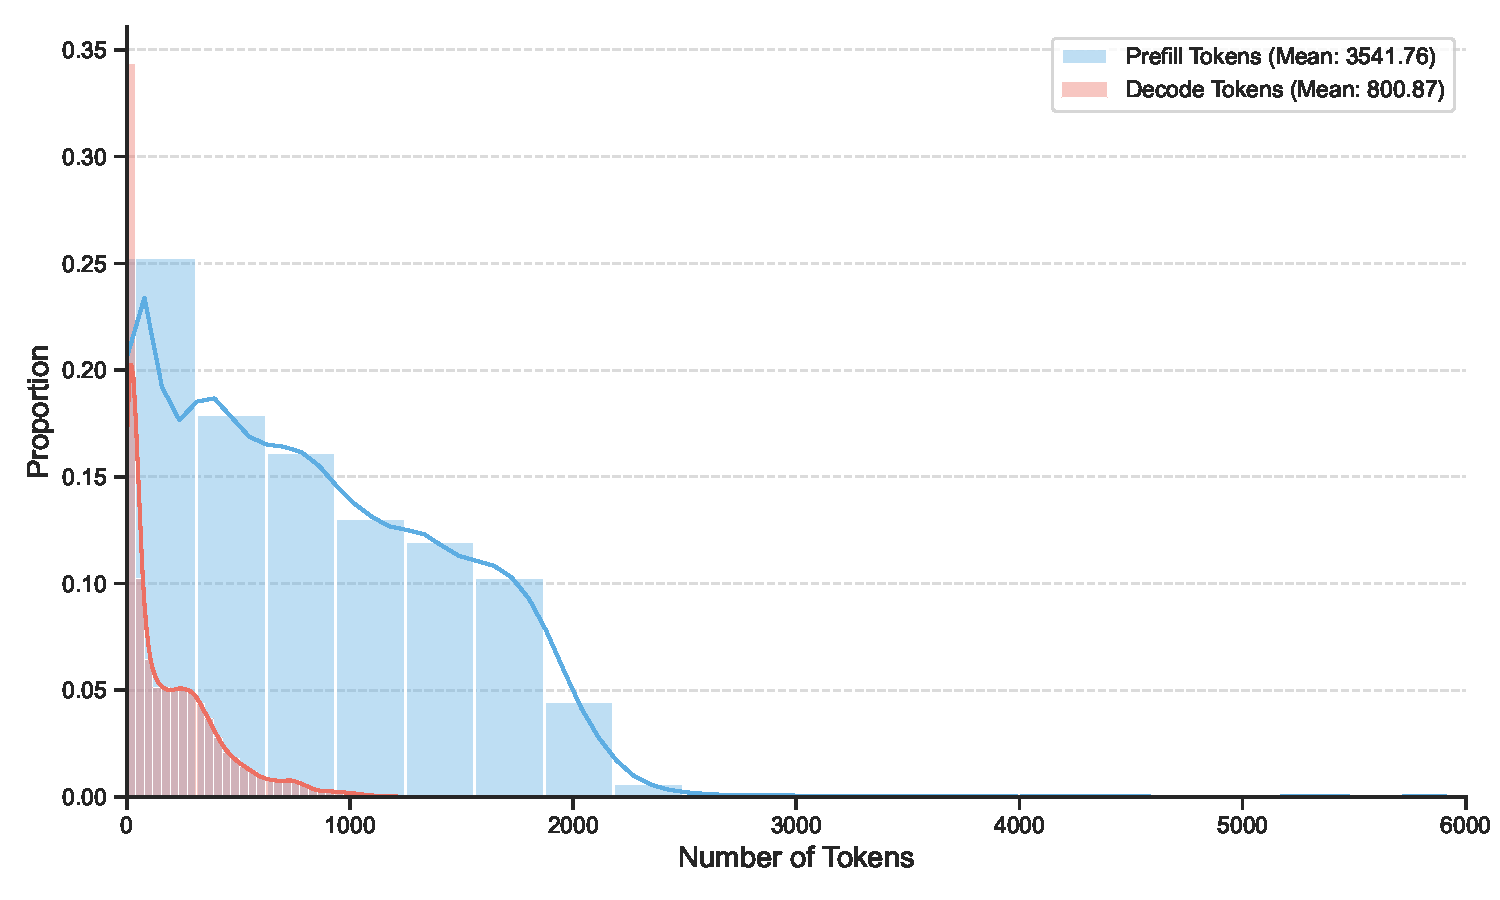
\includegraphics[width=\linewidth]{../figures/5.2.a.pdf}
    \caption{Token Distribution of ShareGPT Dataset}
    \label{fig:top-left}
  \end{subfigure}
  \hfill
  \begin{subfigure}[t]{0.23\textwidth}
    \centering
    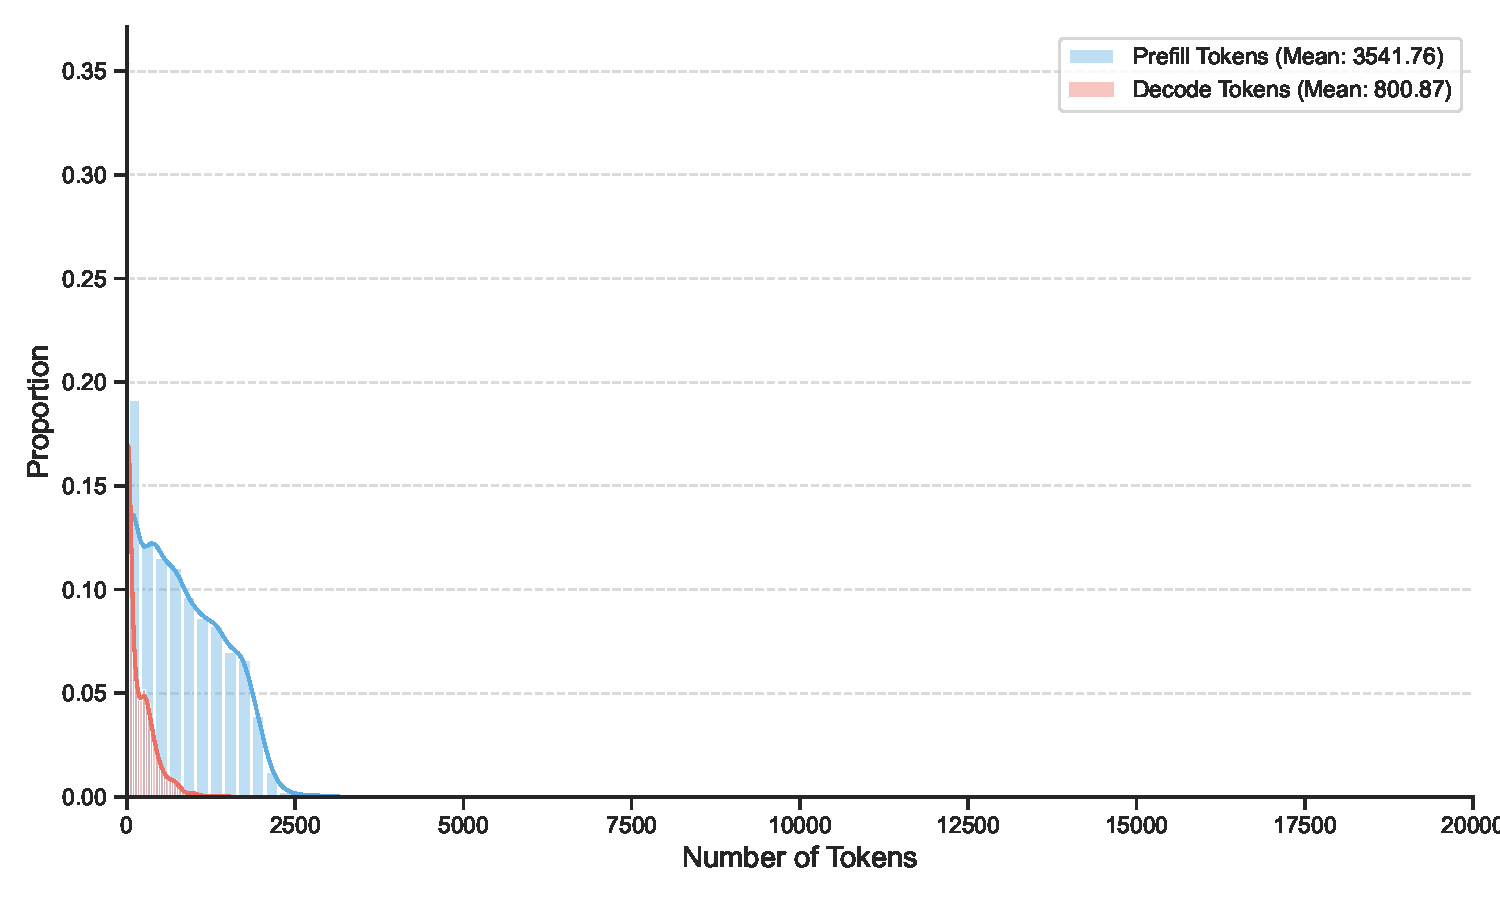
\includegraphics[width=\linewidth]{../figures/5.2.b.pdf}
    \caption{Token Distribution of Wikidata Dataset}
    \label{fig:top-right}
  \end{subfigure}
  \hfill
  \begin{subfigure}[t]{0.23\textwidth}
    \centering
    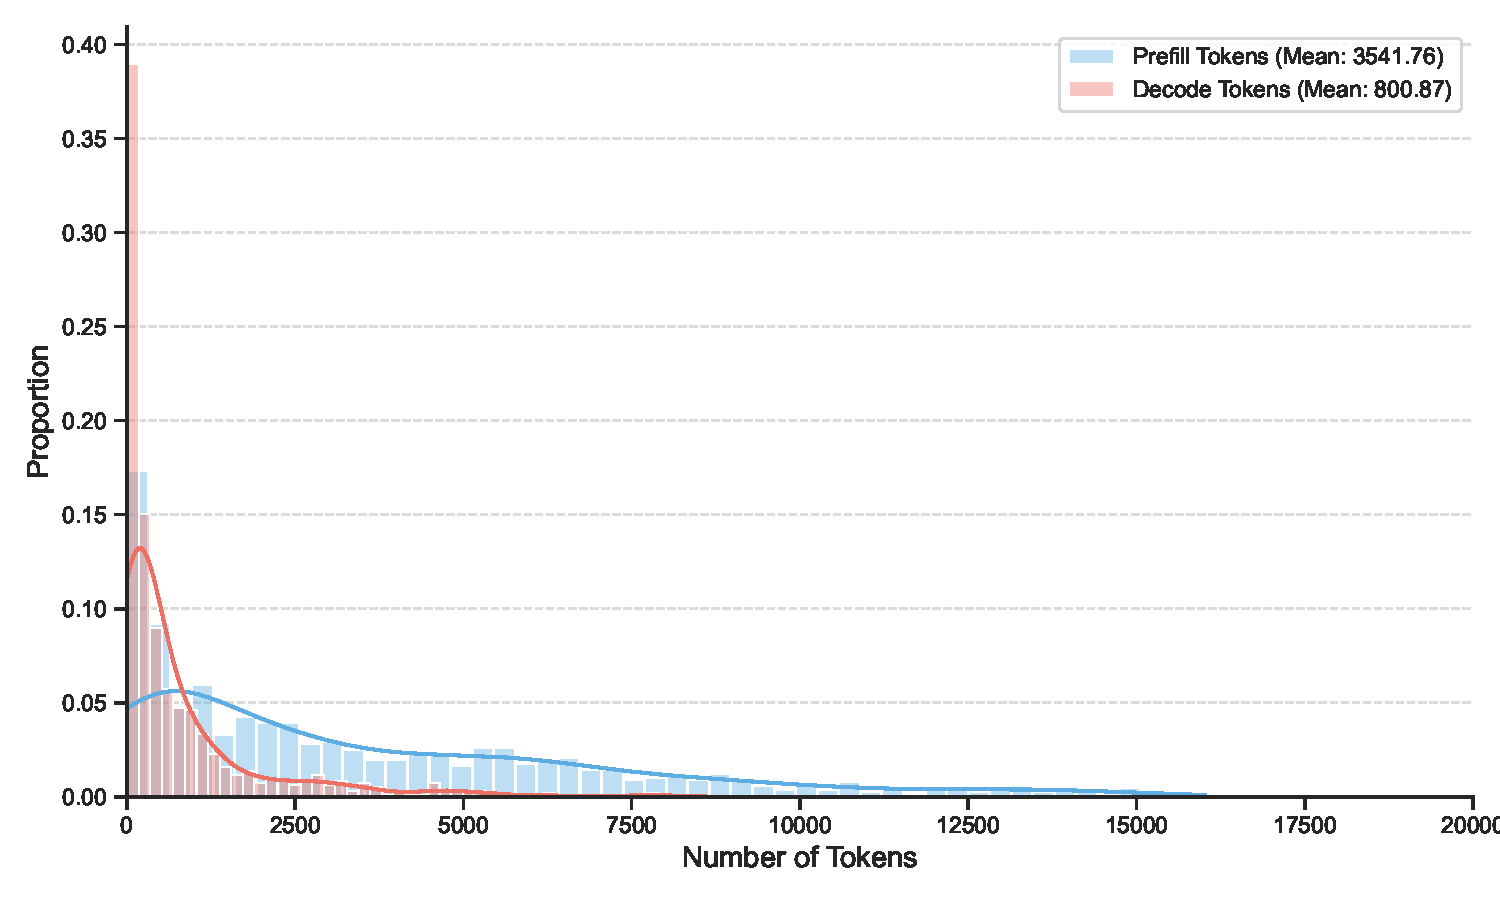
\includegraphics[width=\linewidth]{../figures/5.2.c.pdf}
    \caption{Token Distribution of CodeAgent Dataset}
    \label{fig:bottom-left}
  \end{subfigure}
  \hfill
  \begin{subfigure}[t]{0.23\textwidth}
    \centering
    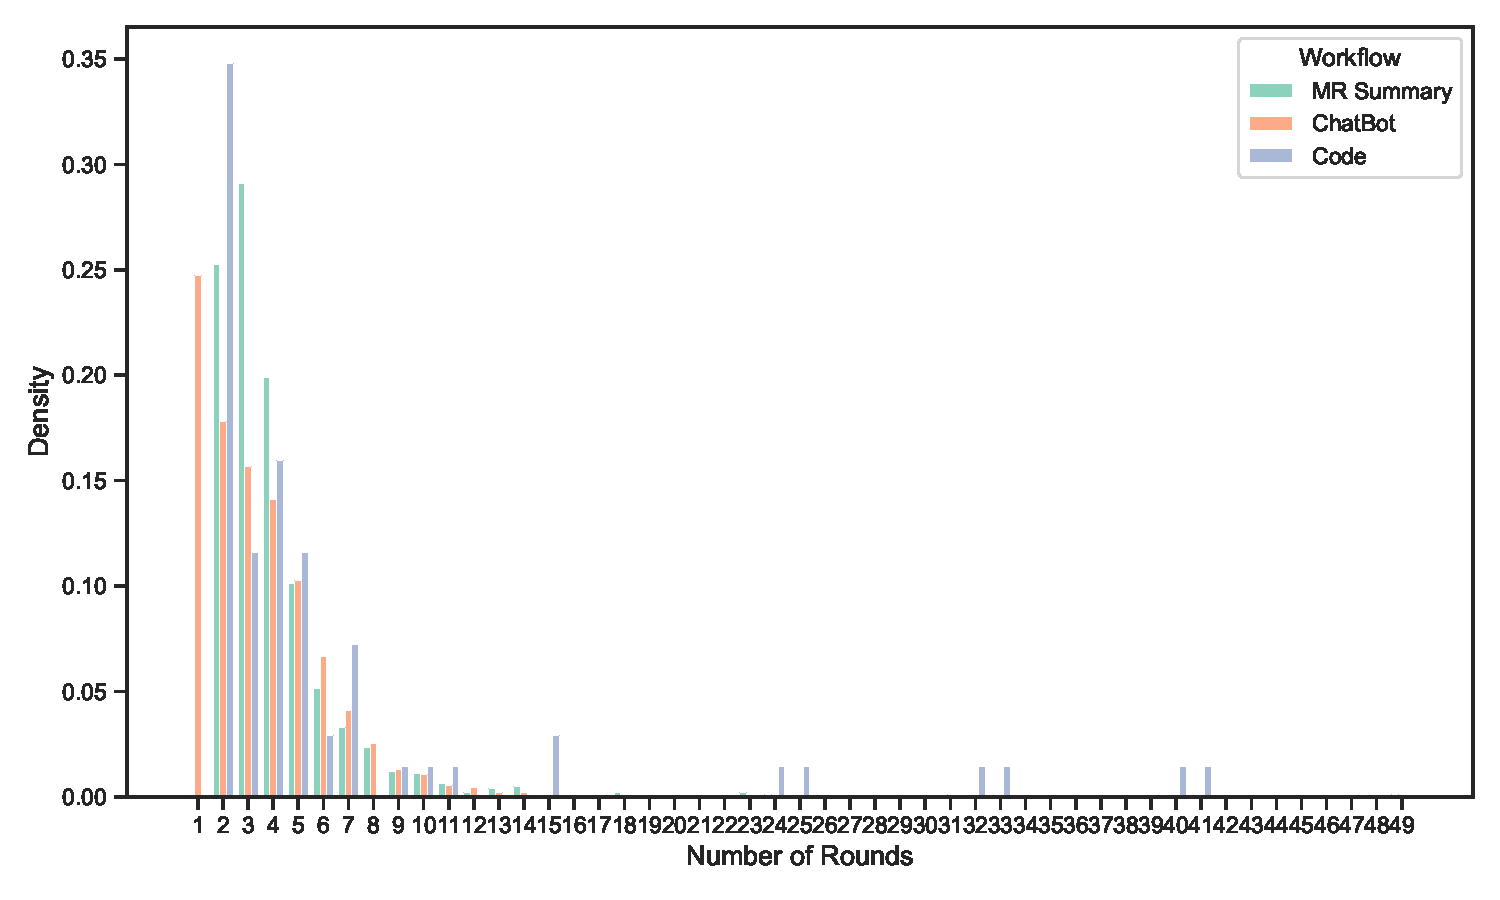
\includegraphics[width=\linewidth]{../figures/5.2.d.pdf}
    \caption{Request Count Distribution of Different Workflows}
    \label{fig:bottom-right}
  \end{subfigure}
  \caption{Feature Distributions of Different Agent Workflows}
  \label{fig:four-images-total}
\end{figure*}

Evaluation proceeds in two steps: first, each of the three workloads
is tested in isolation; then a mixed workload combining all three types
in preset ratios is evaluated. Workflow inter-arrival times follow a
Poisson distribution. All experiments use the Llama3-8B model by
default.

\subsection{Baselines}

We compare RAGS against the following baselines.

\textbf{Round-Robin.}
Serving as our naive baseline, this strategy pairs First-Come-First-Serve (FCFS) 
queuing with round-robin dispatch. It treats all inference requests independently, 
operating entirely without Agent workflow awareness.

\textbf{Parrot~\cite{lin2024parrot}.}
A state-of-the-art LLM serving system that uses semantic variable abstraction to expose
inter-request DAG dependencies to the serving layer.
It employs session affinity routing to maximize KV-cache prefix reuse while aggregating
similar requests to satisfy application-level performance goals.
We faithfully replicate its FCFS queuing and session affinity routing algorithms in our evaluation.

\textbf{Ayo~\cite{tan2025towards}.}
A fine-grained LLM orchestration framework that prioritizes requests based on their
topological depth in the workflow DAG, with round-robin dispatch.
We isolate and implement only its topology-aware queuing and routing logic for comparison.

\subsection{Main Results}

\begin{figure}[t]
  \centering
  \fbox{\rule{0pt}{160pt}\rule{\linewidth}{0pt}}
  \caption{End-to-end performance comparison under three single-type
    workloads at varying request rates.}
  \Description{Placeholder for the single-workload E2E latency figure.}
  \label{fig:exp-e2e-latency}
\end{figure}

Figure~\ref{fig:exp-e2e-latency} shows the end-to-end performance of
each method under the three single-type workloads at varying request
arrival rates.

\textbf{ChatBot (serial).}
At an arrival rate of 20 workflows/s, RAGS achieves up to
\textbf{5.2$\times$} lower mean E2E latency than Round-Robin and Ayo.
For TTFT, Round-Robin's P50 surges to 17\,s under high concurrency,
while RAGS keeps it below 1\,s through RL-based dynamic load balancing
and DynA's priority queuing. RAGS's speedup over Parrot is only
$\approx$1.1$\times$ in this scenario because ChatBot has a fixed
topology with highly regular KV-cache sharing, allowing Parrot's
static prefix-aware routing to effectively exploit the cache; the
headroom for dynamic routing is therefore limited.

\textbf{Map-Reduce Summarization (parallel).}
Since this workflow has a simple two-level topology, the overall gains
of RAGS over baselines are moderate. At 20 workflows/s, RAGS reduces
mean E2E latency by only $\approx$6\% over Round-Robin. Ayo's
topology-based priority essentially degenerates to round-robin because
it cannot distinguish among the many same-level Map nodes. DynA,
however, estimates workflow progress and preferentially schedules
requests about to trigger the Reduce aggregation, partially alleviating
inter-node synchronization blocking.

\textbf{Code Generation Agent (hybrid).}
This workload introduces autonomous feedback-repair loops and is
designed to assess the scheduler's ability to handle highly dynamic
topologies. Parrot causes severe queue congestion in this scenario:
its mean E2E latency reaches 240\,s and P95 tail latency 600\,s,
approximately 3--4$\times$ higher than RAGS. The root cause is that the
repair feedback loops create highly dynamic per-session compute loads,
and static session affinity triggers severe global load imbalance,
causing head-of-line blocking on overloaded instances. Thanks to the
synergy between RL-based dynamic load balancing and DynA's preemptive
scheduling of high-priority requests, RAGS stabilizes mean latency in
the range of 70--85\,s across most load levels, and maintains P95 tail
latency around 200\,s even at 5 workflows/s.

TTFT further reveals the degree of queue congestion under highly
dynamic load. Parrot's P50 TTFT spikes to $\approx$6\,s at
5 workflows/s. RAGS, by jointly optimizing KV-cache reuse and load
balance, keeps P50 TTFT below 0.5\,s under the same heavy load,
demonstrating that two-tier co-design effectively suppresses TTFT
spikes in dynamic workflows.

\textbf{Mixed workload.}
Real production environments feature highly heterogeneous mixed
workloads. We construct a mixed dataset of 500 workflows and vary the
proportions $(x, y, z)$ of ChatBot, Summarization, and Code Agent
workflows. The arrival rate is fixed at 5 workflows/s.
Figure~\ref{fig:exp-e2e-latency-mix} presents mean E2E latency under
four representative mixture ratios.

\begin{figure}[t]
  \centering
  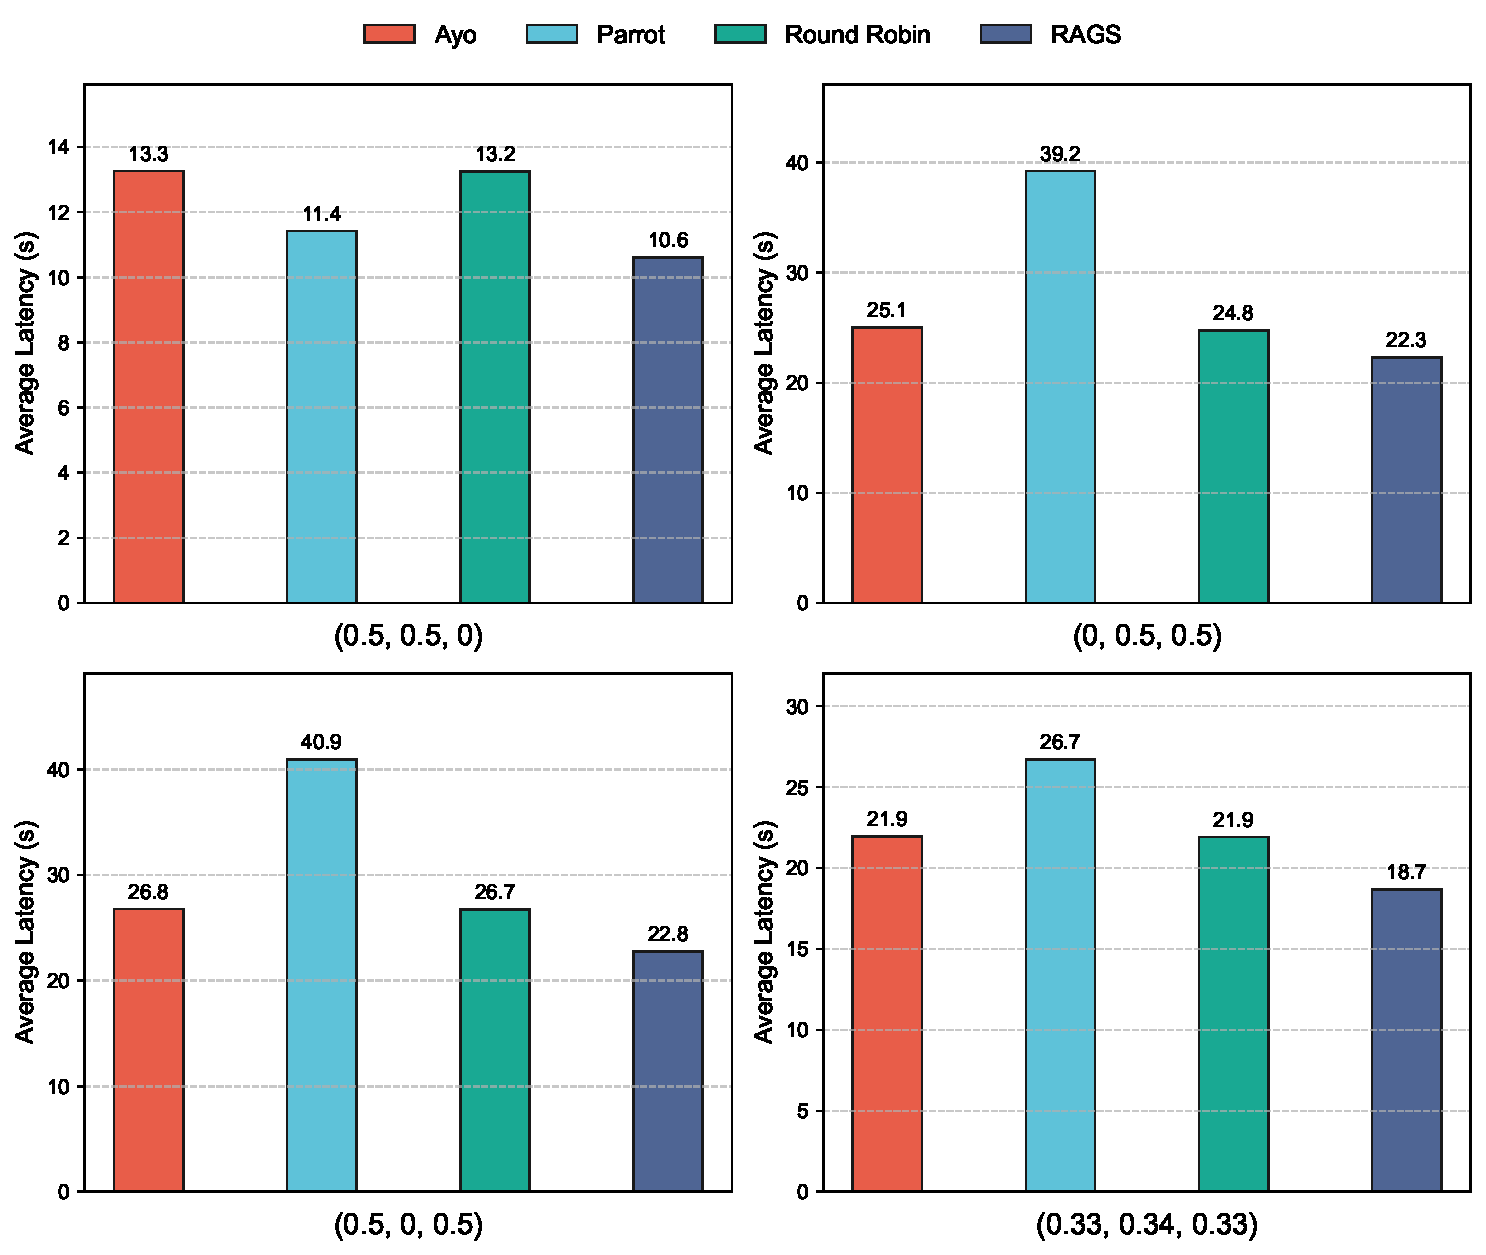
\includegraphics[width=\linewidth]{../figures/5.4.pdf}
  \caption{End-to-end performance comparison under mixed loads.}
  %\Description{A woman and a girl in white dresses sit in an open car.}
  \label{fig:exp-e2e-latency-mix}
\end{figure}

When the mix contains no Code Agent tasks (ratio $(0.5, 0.5, 0)$),
most baselines converge to 11--14\,s, with Parrot achieving 11.4\,s
(second best) and RAGS achieving 10.6\,s (best). Once Code Agent tasks
with complex feedback loops are introduced (e.g., ratios $(0, 0.5, 0.5)$
and $(0.5, 0, 0.5)$), Parrot's latency spikes to $\approx$40\,s,
exposing the inability of static binding to handle high compute
density. Ayo and Round-Robin show similar degradation, confirming
that static topology-depth sorting cannot cope with heterogeneous
concurrent traffic. RAGS achieves 18.7\,s under the balanced mix
$(0.33, 0.34, 0.33)$, which is 14.5\% lower than Ayo and 28.6\% lower than
Parrot, and keeps mean E2E latency below 22.8\,s in every
Code-Agent-inclusive scenario.

\subsection{Hyperparameter Sensitivity}

\subsubsection{Effect of State-Space Bin Width}

\begin{figure}[t]
  \centering
  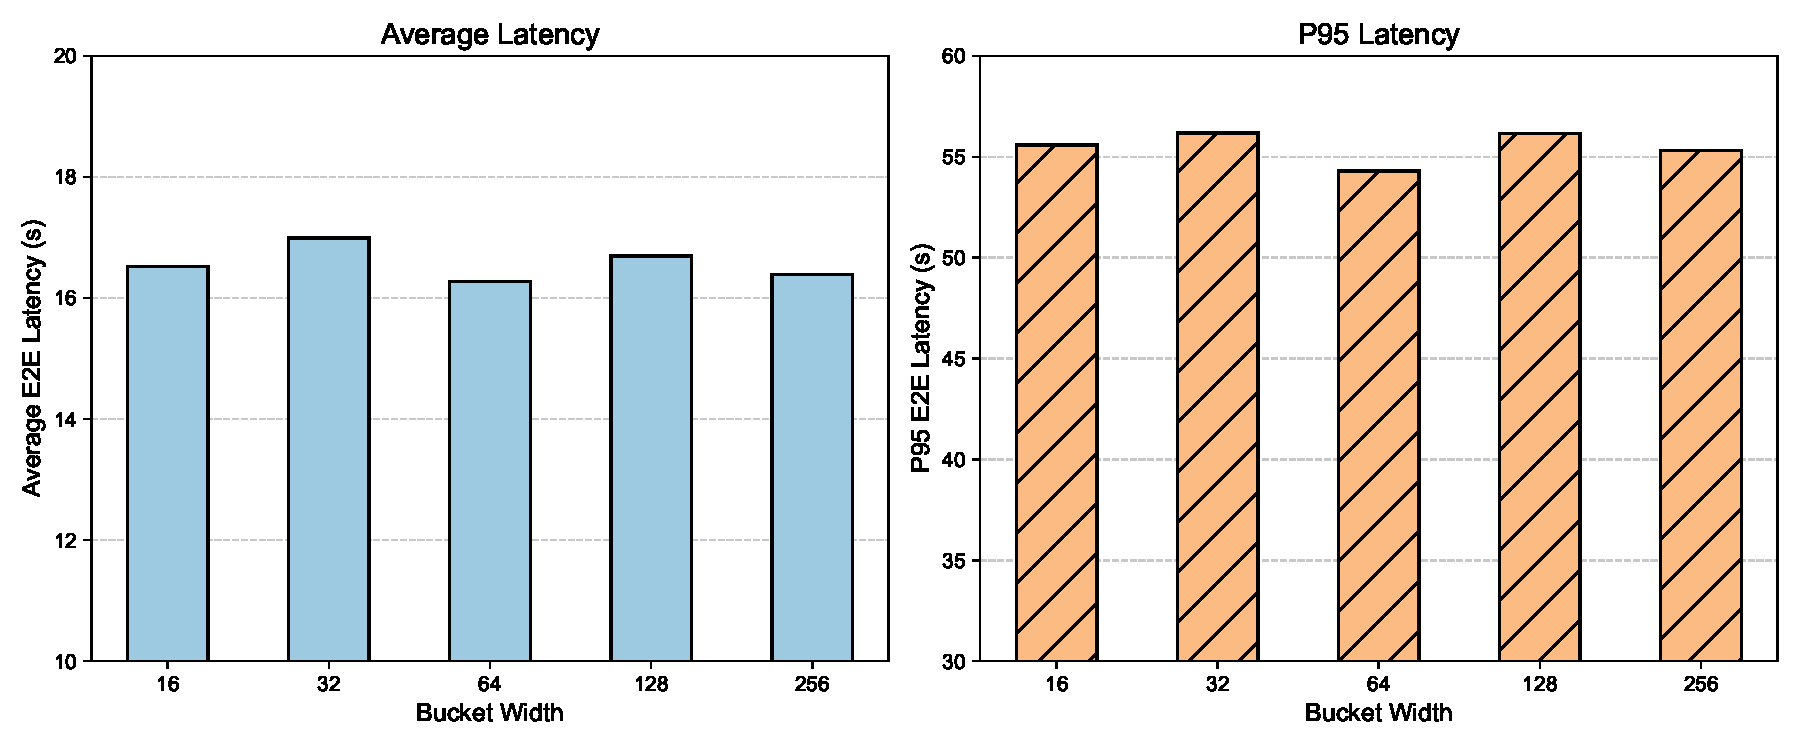
\includegraphics[width=\linewidth]{../figures/5.5.pdf}
  \caption{Effect of bin width on mean E2E latency.}
  \Description{Placeholder for the bin-width ablation figure.}
  \label{fig:ablation-1}
\end{figure}

Figure~\ref{fig:ablation-1} illustrates the impact of the load histogram's bin width 
on the mean E2E latency. An excessively narrow bin width results in sparse state representations, 
which hinders the convergence of the RL algorithm. Conversely, an overly broad bin width obscures 
fine-grained load variations across different instances. Empirical results indicate that a bin 
width of 64 strikes an optimal trade-off between representation fidelity and learning efficiency; 
thus, it is adopted as the default configuration.

\subsection{Ablation Studies}

To quantify the individual contributions of the queuing and dispatch
components, we run an ablation on the mixed workload
(ChatBot:Summarization:Code\,=\,0.33:0.34:0.33) at varying arrival
rates, comparing three configurations:
(1)~\textbf{RAGS}: full system (DynA + RL dispatch);
(2)~\textbf{RAGS w/o DynA}: FCFS queuing + RL dispatch;
(3)~\textbf{RAGS w/o RL}: DynA queuing + Round-Robin dispatch.

\begin{figure}[t]
  \centering
  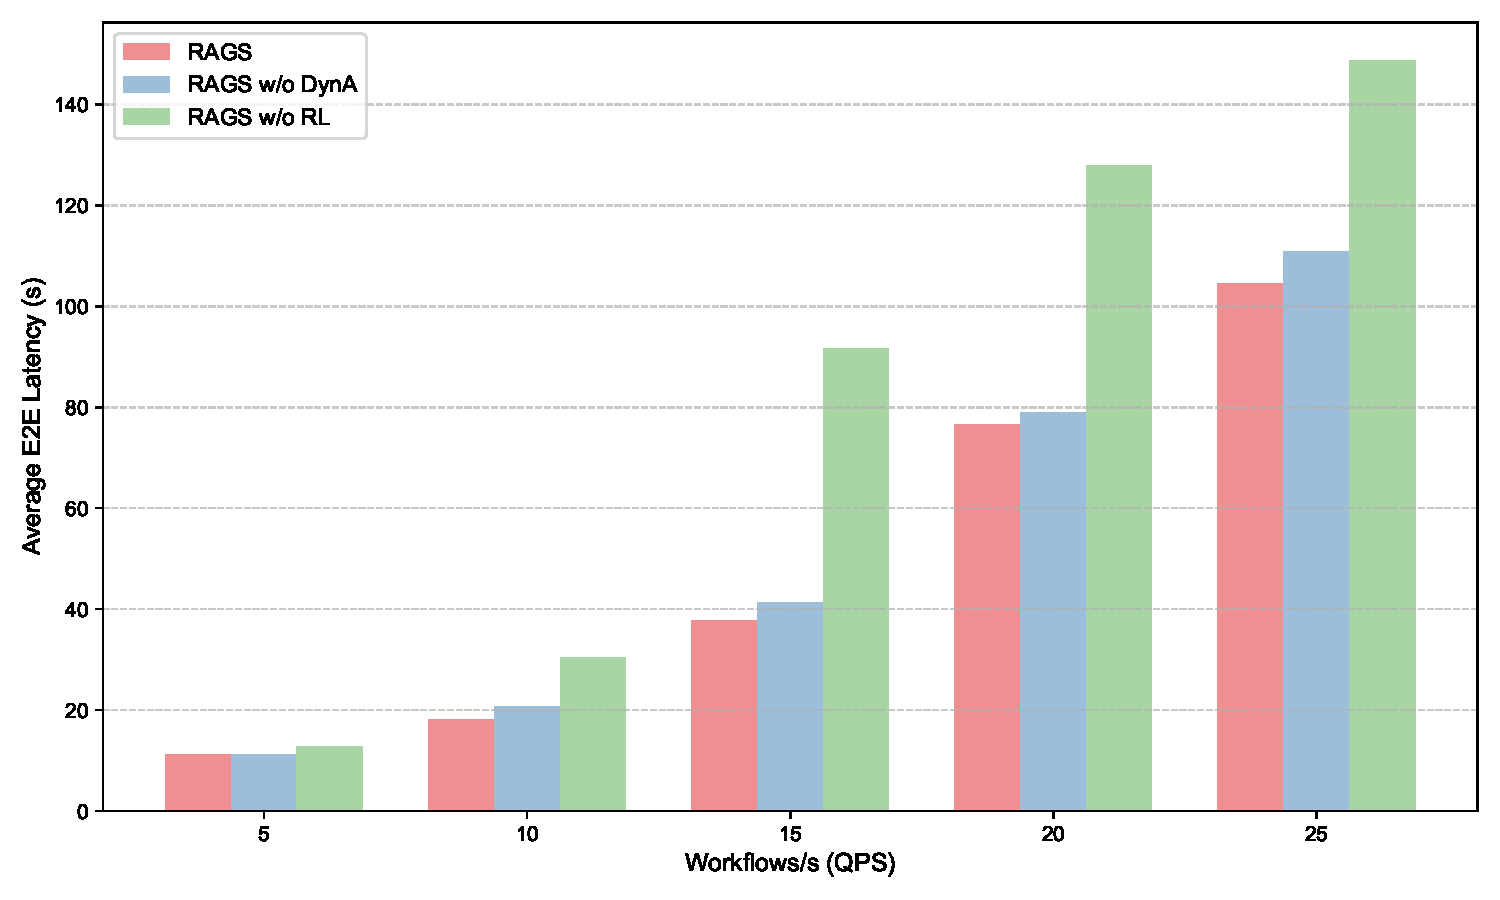
\includegraphics[width=\linewidth]{../figures/5.6.pdf}
  \caption{Component ablation under mixed workload.}
  \Description{Placeholder for the component ablation figure.}
  \label{fig:ablation-2}
\end{figure}

As shown in Figure~\ref{fig:ablation-2}, performance differences
are small at low arrival rates (RAGS: 11.206\,s, RAGS w/o DynA:
11.205\,s, RAGS w/o RL: 12.867\,s) but widen significantly at high
loads. At the peak arrival rate, RAGS achieves 104.557\,s; removing
DynA raises latency to 110.804\,s; removing RL dispatch degrades
latency further to 148.758\,s.

These results lead to three conclusions. First, RL dispatch is the
dominant contributor: removing it increases peak mean latency by
$\approx$42.27\%, confirming that its benefit scales with system load.
Second, DynA also provides non-trivial gains: at a medium arrival rate
RAGS w/o DynA's latency is $\approx$14.8\% higher than RAGS
(20.782\,s vs.\ 18.104\,s), showing that workflow-progress-aware
priority ordering effectively reduces head-of-line blocking.
Third, the two components are complementary: DynA ensures that
critical requests enter the dispatch stage first, while RL global load
balancing prevents those requests from encountering secondary queuing
inside LLM engines.

\subsection{Heterogeneous Cluster Evaluation}
\label{subsec:chap4-heterogeneous}

\begin{figure}[t]
  \centering
  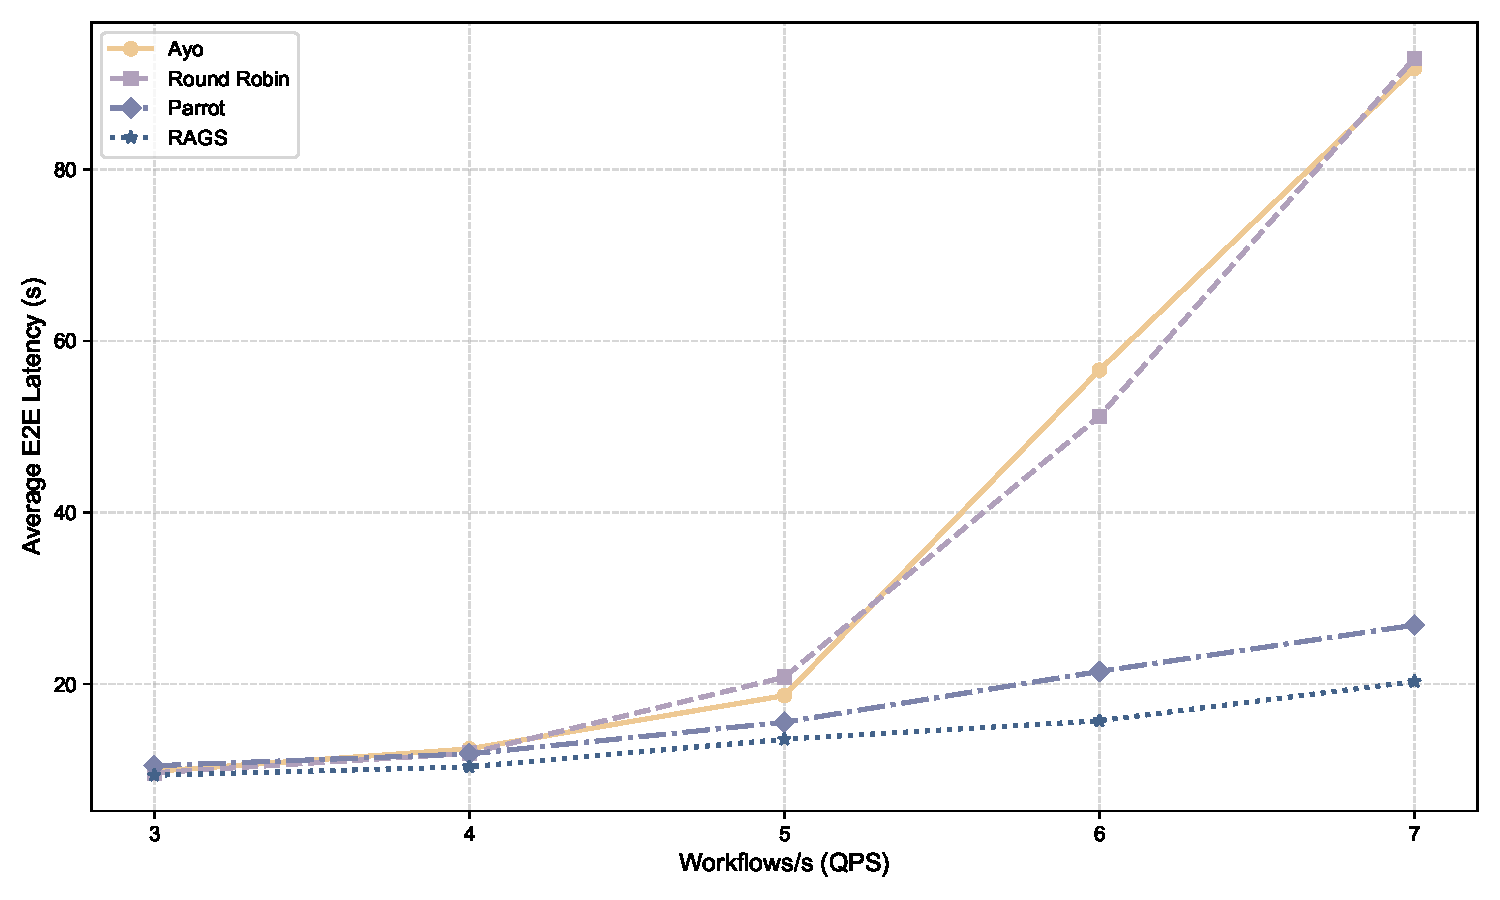
\includegraphics[width=\linewidth]{../figures/5.7.pdf}
  \caption{Heterogeneous GPU cluster evaluation results.}
  \Description{Placeholder for the heterogeneous cluster figure.}
  \label{fig:heterogeneous-comparison}
\end{figure}

To validate RAGS on a heterogeneous GPU cluster, we run experiments on
a 4-GPU cluster with 2 NVIDIA A100s and 2 NVIDIA H100s. Since
complete performance benchmarks for Meta-Llama-3-8B on H100 are not
yet available, all instances deploy meta-llama/Llama-2-7b-hf. A100
and H100 differ significantly in compute throughput and memory
bandwidth, so the scheduler must sense hardware heterogeneity while
avoiding resource waste from unbalanced allocation.

As shown in Figure~\ref{fig:heterogeneous-comparison}, all methods
exhibit increasing mean E2E latency as the arrival rate rises from
3 to 7 workflows/s, but with markedly different slopes. Round-Robin
ignores GPU heterogeneity and distributes evenly, turning the weaker
A100 instances into system bottlenecks; its latency surges above 80\,s
at high concurrency. Parrot's static session-binding also lacks
hardware-awareness: routing computationally intensive requests to
weaker A100 instances easily triggers severe local overload.

RAGS maintains the lowest mean E2E latency at all load levels. Its
advantage stems from the joint encoding of GPU type and instance load
in the RL state space, which allows the policy to implicitly sense
inter-instance compute differences and adaptively balance hardware
performance with global load distribution. At the peak arrival rate
of 7 workflows/s, RAGS reduces mean E2E latency by approximately
30\%--40\% compared with Round-Robin and Parrot, validating its
effectiveness and generalizability in heterogeneous inference clusters.

%%
%% Related Work
\section{Related Work}\label{sec:related-work}

\textbf{LLM Inference Engines.}
vLLM~\cite{kwon2023efficient} introduces PagedAttention to manage KV cache
with OS-style virtual memory paging, greatly reducing memory fragmentation
and improving GPU utilization.  SGLang~\cite{zheng2024sglang} further
proposes RadixAttention, indexing all historical KV caches in a radix tree
to enable fine-grained cross-request prefix reuse and cache-aware routing.
Sarathi-Serve~\cite{agrawal2024taming} mitigates prefill--decode interference
via chunked prefills, while Orca~\cite{yu2022orca} pioneered continuous
batching to keep GPUs fully occupied.  These systems optimize single-turn
request serving but lack mechanisms to model multi-step workflow
dependencies inherent in agent workloads.

\textbf{LLM Agent Serving Systems.}
Parrot~\cite{lin2024parrot} is among the first to address agent workflow
scheduling: it introduces \emph{semantic variables} to expose inter-request
data-flow to the serving layer and adopts session-affinity routing to
maximize KV cache reuse across correlated requests.  Ayo~\cite{tan2025towards}
decomposes complex LLM applications into primitive-level dataflow graphs
and co-schedules LLM and non-LLM stages in a pipeline, cutting end-to-end
latency.  Autellix~\cite{luo2025autellix} elevates the full agent program
to the scheduling unit and proposes PLAS/ATLAS—multi-level feedback queue
schedulers that use accumulated execution time on the critical path to
mitigate head-of-line blocking.  KVFlow~\cite{pan2025kvflow} focuses on
cache management for multi-agent workflows: it builds an agent execution
graph, assigns priority to cache nodes based on estimated reuse distance,
and employs asynchronous prefetching together with a future-reuse-aware
eviction policy to raise cache hit rates.  HexGen-Flow~\cite{peng2025hexgen}
proposes a two-level SLO-aware scheduler for Text-to-SQL pipelines,
decomposing end-to-end budgets proportionally and using urgency-based
preemption; however, it is tightly coupled to a specific pipeline structure
and does not generalize to arbitrary agent topologies.

\textbf{RL for Cluster Scheduling.}
DeepRM~\cite{mao2016resource} and DL2~\cite{peng2021dl2} demonstrate the
effectiveness of deep RL for resource scheduling in DNN training clusters.
TORTA~\cite{du2025temporal} applies RL to LLM inference traffic routing
across regions, dynamically adjusting per-window routing ratios.  Unlike
these works, RAGS applies RL to \emph{agent workflow} routing, explicitly
encoding workflow-level dependency states and KV cache residency to drive
adaptive global dispatching.

%%
%% The acknowledgments section is defined using the "acks" environment
%% (and NOT an unnumbered section). This ensures the proper
%% identification of the section in the article metadata, and the
%% consistent spelling of the heading.
%% \begin{acks}
%% To Robert, for the bagels and explaining CMYK and color spaces.
%% \end{acks}

%%
%% The next two lines define the bibliography style to be used, and
%% the bibliography file.
\bibliographystyle{ACM-Reference-Format}
\bibliography{../ref/refs}


%% Appendix (disabled)
\iffalse
%% If your work has an appendix, this is the place to put it.
\appendix

\section{Research Methods}

\subsection{Part One}

Lorem ipsum dolor sit amet, consectetur adipiscing elit. Morbi
malesuada, quam in pulvinar varius, metus nunc fermentum urna, id
sollicitudin purus odio sit amet enim. Aliquam ullamcorper eu ipsum
vel mollis. Curabitur quis dictum nisl. Phasellus vel semper risus, et
lacinia dolor. Integer ultricies commodo sem nec semper.

\subsection{Part Two}

Etiam commodo feugiat nisl pulvinar pellentesque. Etiam auctor sodales
ligula, non varius nibh pulvinar semper. Suspendisse nec lectus non
ipsum convallis congue hendrerit vitae sapien. Donec at laoreet
eros. Vivamus non purus placerat, scelerisque diam eu, cursus
ante. Etiam aliquam tortor auctor efficitur mattis.

\section{Online Resources}

Nam id fermentum dui. Suspendisse sagittis tortor a nulla mollis, in
pulvinar ex pretium. Sed interdum orci quis metus euismod, et sagittis
enim maximus. Vestibulum gravida massa ut felis suscipit
congue. Quisque mattis elit a risus ultrices commodo venenatis eget
dui. Etiam sagittis eleifend elementum.

Nam interdum magna at lectus dignissim, ac dignissim lorem
rhoncus. Maecenas eu arcu ac neque placerat aliquam. Nunc pulvinar
massa et mattis lacinia.
\fi

\end{document}
\endinput
%%
%% End of file `sample-sigconf.tex'.
